%% ============================================================
%%  Дипломная (бакалаврская) работа
%%  «Детекция цвета, номеров, марки машины
%%   по материалам видеокамеры»
%%  МФТИ, 2025
%%  Компилируется: pdfLaTeX
%% ============================================================
\documentclass[10pt,a4paper]{report}

%% ── Кодировка и язык ──────────────────────────────────────
\usepackage[T2A]{fontenc}
\usepackage[utf8]{inputenc}
\usepackage[russian,english]{babel}

%% ── Юникод-символы, не определённые в pdfLaTeX по умолчанию ──
\DeclareUnicodeCharacter{2194}{\ensuremath{\leftrightarrow}}  % ↔
\DeclareUnicodeCharacter{2192}{\ensuremath{\rightarrow}}      % →
\DeclareUnicodeCharacter{00B0}{\ensuremath{{}^\circ}}         % °
\DeclareUnicodeCharacter{00E1}{\'a}                            % á

%% ── Шрифт Times New Roman ─────────────────────────────────
\usepackage{newtxtext}

%% ── Поля страницы ─────────────────────────────────────────
\usepackage[left=30mm,right=15mm,top=20mm,bottom=20mm]{geometry}

%% ── Математика ────────────────────────────────────────────
\usepackage{amsmath,amssymb,mathtools}
\usepackage{newtxmath}

%% ── Графика и таблицы ─────────────────────────────────────
\usepackage{graphicx}
\graphicspath{{./}{figs/}}
\usepackage{booktabs}
\usepackage{array}
\usepackage{tabularx}
\usepackage{multirow}
\usepackage{colortbl}
\usepackage[table]{xcolor}
\usepackage{pdfpages}

%% ── TikZ для схем ─────────────────────────────────────────
\usepackage{tikz}
\usetikzlibrary{shapes.geometric, arrows.meta, positioning,
                fit, backgrounds, calc, chains}

%% ── Оформление ────────────────────────────────────────────
\usepackage{indentfirst}
\usepackage{setspace}
\usepackage{enumitem}
\usepackage{caption}
\usepackage{subcaption}
%% Рисунок: по центру, «Рисунок X – Название»
\captionsetup[figure]{
  justification=centering,
  labelsep=endash
}
%% Таблица: слева, без абзацного отступа, «Таблица X – Название»
\captionsetup[table]{
  justification=raggedright,
  singlelinecheck=false,
  labelsep=endash
}
\usepackage{float}
\usepackage{fancybox}
\usepackage{tcolorbox}

%% ── Гиперссылки ───────────────────────────────────────────
\usepackage[hidelinks,unicode]{hyperref}

%% ── Микротипографика и предотвращение вылезания строк ─────
\usepackage{microtype}
\setlength{\emergencystretch}{1.5em}

%% ── Контроль висячих строк и заполнения страниц ───────────
\clubpenalty=10000          % запрет одиночной строки абзаца ВНИЗУ страницы
\widowpenalty=10000         % запрет одиночной строки абзаца ВВЕРХУ страницы
\displaywidowpenalty=10000  % то же рядом с выключными формулами
\brokenpenalty=10000        % не разрывать страницу на переносе слова
\usepackage{needspace}      % \needspace{N\baselineskip} --- держать блок целиком
\raggedbottom               % не растягивать вертикаль (важно для страниц с рисунками)

%% ── Переименование подписей ──────────────────────────────
\addto\captionsenglish{\renewcommand{\figurename}{Рисунок}}
\addto\captionsrussian{\renewcommand{\figurename}{Рисунок}}
\addto\captionsenglish{\renewcommand{\tablename}{Таблица}}
\addto\captionsrussian{\renewcommand{\tablename}{Таблица}}
\addto\captionsenglish{\renewcommand{\contentsname}{Содержание}}
\addto\captionsrussian{\renewcommand{\contentsname}{Содержание}}
\addto\captionsrussian{\renewcommand{\bibname}{Список использованных источников}}
\addto\captionsenglish{\renewcommand{\bibname}{Список использованных источников}}

%% ── Стиль заголовков глав и разделов (14 пт, жирный, по центру) ──
\usepackage{titlesec}
\titleformat{\chapter}[block]
  {\normalfont\normalsize\bfseries\centering}{\thechapter}{1em}{}
\titlespacing*{\chapter}{0pt}{-10pt}{20pt}
\titleformat{\section}
  {\normalfont\normalsize\bfseries\centering}{\thesection}{1em}{}
\titleformat{\subsection}
  {\normalfont\normalsize\bfseries\centering}{\thesubsection}{1em}{}
\titleformat{\subsubsection}
  {\normalfont\normalsize\bfseries\centering}{\thesubsubsection}{1em}{}

%% ── Межстрочный интервал 1.5 ──────────────────────────────
\onehalfspacing

%% ── Абзацный отступ 1.25 см ──────────────────────────────
\setlength{\parindent}{1.25cm}

%% ── Глубина оглавления: до пунктов включительно ──────────
\setcounter{tocdepth}{3}

%% ── Нумерация по главам ───────────────────────────────────
\numberwithin{equation}{chapter}
\numberwithin{figure}{chapter}
\numberwithin{table}{chapter}

%% ── Цвета для схем ────────────────────────────────────────
\definecolor{bluenode}{RGB}{52,101,164}
\definecolor{greennode}{RGB}{30,130,76}
\definecolor{orangenode}{RGB}{200,100,20}
\definecolor{graynode}{RGB}{100,100,110}
\definecolor{lightblue}{RGB}{210,228,255}
\definecolor{lightgreen}{RGB}{210,240,215}
\definecolor{lightorange}{RGB}{255,230,200}
\definecolor{lightgray}{RGB}{235,235,240}
\definecolor{rowgray}{RGB}{245,245,248}

%% ── TikZ стили ────────────────────────────────────────────
\tikzset{
  block/.style={
    rectangle, rounded corners=4pt, minimum width=3cm,
    minimum height=1cm, text centered, text width=3.2cm,
    draw, font=\small
  },
  blk/.style={block, fill=lightblue,  draw=bluenode,   thick},
  grn/.style={block, fill=lightgreen, draw=greennode,  thick},
  org/.style={block, fill=lightorange,draw=orangenode, thick},
  gry/.style={block, fill=lightgray,  draw=graynode,   thick},
  arr/.style={-{Stealth[length=6pt]}, thick},
  darr/.style={arr, dashed},
  lbl/.style={font=\footnotesize, midway, right=2pt}
}

% ─────────────────────────────────────────────────────────────
\begin{document}

%% =====================  ТИТУЛЬНЫЙ ЛИСТ (официальный PDF)  =====================

\includepdf[pages=1]{titlepage.pdf}
\setcounter{page}{1}   % титул не нумеруется; аннотация --- страница 1

%% =====================  АННОТАЦИЯ  ==========================
\chapter*{Аннотация}
\addcontentsline{toc}{chapter}{Аннотация}

\noindent\textbf{Ключевые слова:} детекция транспортных средств, распознавание
номерных знаков, классификация цвета и типа кузова, YOLO26, ResNet18,
EasyOCR, transfer learning, глубокое обучение.

\textbf{Цель работы}~--- разработка системы автоматического определения
характеристик транспортных средств (номерной знак, цвет, тип кузова) по
видеопотоку.

\textbf{Задачи:} анализ методов детекции и классификации, выбор и обоснование
архитектур глубокого обучения, подготовка датасетов, обучение и оценка
моделей, интеграция в единый конвейер обработки видео.

\textbf{Результаты:} предложена конвейерная архитектура (YOLO26n~--- детекция
ТС и номеров, ResNet18~--- цвет и тип кузова, EasyOCR~--- OCR кириллицы).
Детектор номеров достиг mAP@0.50\,=\,0.9669; классификатор цвета~---
Accuracy\,=\,0.936; типа кузова~--- Accuracy\,=\,0.830;
EasyOCR~--- CRR\,=\,0.750 на реальных данных.

\textbf{Рекомендации:} заменить EasyOCR специализированным OCR для российских
номеров и расширить набор классов атрибутов.

%% =====================  СОДЕРЖАНИЕ  =========================
\tableofcontents

%% =====================  ОБОЗНАЧЕНИЯ И СОКРАЩЕНИЯ  ===========
\chapter*{Обозначения и сокращения}
\addcontentsline{toc}{chapter}{Обозначения и сокращения}

\begin{tabular}{@{}lp{0.72\textwidth}@{}}
ANPR      & Automatic Number Plate Recognition --- автоматическое распознавание номерных знаков \\[4pt]
BN        & Batch Normalization --- пакетная нормализация \\[4pt]
CNN       & Convolutional Neural Network --- сверточная нейронная сеть \\[4pt]
CRR       & Character Recognition Rate --- доля верно распознанных символов \\[4pt]
DCNN      & Deep CNN --- глубокая сверточная нейронная сеть \\[4pt]
FPN       & Feature Pyramid Network --- сеть пирамиды признаков \\[4pt]
GAP       & Global Average Pooling \\[4pt]
IoU       & Intersection over Union --- пересечение по объединению \\[4pt]
LR        & Learning Rate --- скорость обучения \\[4pt]
mAP       & mean Average Precision --- средняя точность по классам \\[4pt]
OCR       & Optical Character Recognition --- оптическое распознавание символов \\[4pt]
ReLU      & Rectified Linear Unit \\[4pt]
SGD       & Stochastic Gradient Descent --- стохастический градиентный спуск \\[4pt]
SiLU      & Sigmoid Linear Unit (Swish) \\[4pt]
ТС        & Транспортное средство \\[4pt]
VMMR      & Vehicle Make and Model Recognition --- распознавание марки и модели ТС \\[4pt]
YOLO      & You Only Look Once --- одноэтапный детектор объектов \\
\end{tabular}

%% =============================================================
%%  ГЛАВА 1 --- ВВЕДЕНИЕ
%% =============================================================
\chapter*{Введение}
\addcontentsline{toc}{chapter}{Введение}

\section*{Актуальность задачи}
\addcontentsline{toc}{section}{Актуальность задачи}

В настоящее время анализ видеоизображений широко применяется для мониторинга
дорожного движения, обеспечения безопасности и контроля доступа на объекты.
Объём видеоданных постоянно растёт, что делает ручную
обработку информации неэффективной и трудоёмкой.

Практический интерес представляет автоматическое определение характеристик
автомобиля: государственного регистрационного знака, марки, модели и цвета.
Эти данные применяются в задачах контроля проезда, поиска транспортных средств
и учёта трафика. Однако качество видеозаписей часто
ограничено низким разрешением, изменениями освещённости,
погодными условиями и движением объектов.

\section*{Цель и задачи работы}
\addcontentsline{toc}{section}{Цель и задачи работы}

\textbf{Объект исследования}~--- видеоизображения транспортных средств,
полученные в реальных условиях эксплуатации.

\textbf{Предмет исследования}~--- методы и алгоритмы автоматического определения
характеристик транспортных средств (номерной знак, цвет кузова, тип кузова)
на основе глубокого обучения.

\textbf{Цель}~--- разработка системы автоматического определения цвета,
типа кузова и номерного знака автомобиля по видеопотоку.

\textbf{Задачи:}
\begin{enumerate}
  \item Провести анализ существующих методов детекции ТС, ANPR, VMMR и определения цвета.
  \item Выбрать и обосновать архитектуры моделей для каждой подзадачи.
  \item Подготовить обучающие датасеты.
  \item Обучить и оценить модели детекции номеров, классификаторы цвета и типа кузова.
  \item Интегрировать модели в единый конвейер обработки видео.
  \item Провести сравнительный эксперимент ResNet18, ResNet50 и EfficientNet-B0.
\end{enumerate}

\textbf{Методы исследования:} анализ научно-технической
литературы; методы глубокого обучения (сверточные нейронные сети, transfer
learning); экспериментальный метод~--- сравнительное тестирование архитектур
ResNet18, ResNet50 и EfficientNet-B0; метрический анализ качества моделей (mAP, Accuracy,
CRR, IoU).

\textbf{Научно-теоретическая значимость} работы состоит в систематизации
и сравнительном анализе современных методов детекции транспортных средств,
автоматического распознавания номерных знаков, классификации типа кузова и цвета;
в обосновании эффективности конвейерной архитектуры на основе transfer learning
для задач видеоаналитики транспорта.

\textbf{Практическая значимость} работы состоит в разработке работоспособного
прототипа системы для автоматизации анализа транспортных потоков по видеоизображениям.

\textbf{Апробация результатов.} Результаты работы не выносились на публикацию
или конференции; они представлены в форме выпускной квалификационной работы.

\section*{Постановка задачи}
\addcontentsline{toc}{section}{Постановка задачи}

Задача анализа транспортных средств по видеоданным представляется как
последовательность следующих этапов:

\begin{enumerate}[nosep]
  \item детекция автомобиля в кадре;
  \item локализация номерного знака внутри области автомобиля;
  \item оптическое распознавание символов номера;
  \item классификация визуальных атрибутов: цвет и тип кузова.
\end{enumerate}

Формально результат детекции объектов на изображении:
\begin{equation*}
  D = \bigl\{(b_i,\, c_i,\, p_i)\bigr\}_{i=1}^{N},
\end{equation*}
где $b_i = (x_i, y_i, w_i, h_i)$~--- ограничивающий прямоугольник,
$c_i$~--- класс объекта, $p_i$~--- уверенность детекции.

Качество локализации оценивается через Intersection over Union:
\begin{equation*}
  \mathrm{IoU} = \frac{S(B_{\mathrm{pred}} \cap B_{\mathrm{gt}})}
                      {S(B_{\mathrm{pred}} \cup B_{\mathrm{gt}})}.
\end{equation*}

\chapter{Обзор существующих методов}

\section{Детекция транспортных средств}

\subsection{Сравнение подходов к детекции}

Эволюция методов детекции объектов прошла несколько этапов.
Таблица~\ref{tab:detectors} суммирует основные подходы.

\begin{table}[H]
\centering
\caption{Сравнение методов детекции объектов}
\label{tab:detectors}
\rowcolors{2}{rowgray}{white}
\begin{tabularx}{\textwidth}{l>{\raggedright\arraybackslash}X>{\raggedright\arraybackslash}Xcc}
\toprule
\textbf{Метод} & \textbf{Принцип} & \textbf{Достоинства} & \textbf{mAP} & \textbf{FPS} \\
\midrule
HOG+SVM       & Ручные признаки, скользящее окно   & Прост в реализации, нет GPU  & низкий & 5--15 \\
Haar-каскады  & Каскад слабых классификаторов      & Очень быстрые на CPU          & низкий & 30+ \\
Faster R-CNN  & Двухэтапная сеть, RPN+cls          & Высокая точность              & высокий & 5--15 \\
SSD           & Одноэтапная, anchor-based          & Баланс скорости и точности    & средний & 46+ \\
\textbf{YOLO26n} & \textbf{Одноэтапная, anchor-free, NMS-free} & \textbf{Скорость + точность} & \textbf{высокий} & \textbf{100+} \\
\bottomrule
\end{tabularx}
\end{table}

\subsection{Двухэтапные детекторы (Faster R-CNN)}

Детекторы семейства Faster R-CNN работают в два этапа: Region Proposal Network
генерирует кандидаты, затем классификационная голова уточняет координаты.
Подход обеспечивает высокую точность, но требователен к вычислительным ресурсам
и не обеспечивает скорость, достаточную для обработки видео в реальном времени.

\subsection{Одноэтапные детекторы (YOLO)}

Семейство YOLO~\cite{survey2021} решает задачу детекции за один проход по сети.
Anchor-free архитектура, CSP-backbone и PAN-FPN neck обеспечивают
работу на GPU со скоростью 100+ FPS при конкурентоспособной точности.
В качестве детектора в работе используется \textbf{YOLO26n}~\cite{yolo26}~---
актуальная модель семейства (2026), которая дополнительно реализует
end-to-end инференс без NMS и отказ от Distribution Focal Loss, что
упрощает экспорт и снижает задержку (см.\ раздел~\ref{sec:yolo26}).

\noindent\textbf{Обоснование выбора:} YOLO26n оптимален для видеопотока
в реальном времени, совместим с форматами ONNX/TensorRT и при меньшем числе
параметров превосходит предыдущее поколение по точности на целевых данных
(сравнение с YOLOv8n~--- подраздел~\ref{subsec:yolo_compare}).

\section{Распознавание номерных знаков (ANPR)}

Типовая ANPR-система включает несколько последовательных этапов~\cite{laroca2018,laroca2021},
схема которых представлена на рисунке~\ref{fig:anpr_flow}.

\begin{figure}[H]
\centering
\resizebox{\linewidth}{!}{%
\begin{tikzpicture}[node distance=0.7cm, every node/.style={font=\small}]
  \node[blk, text width=2.6cm] (cam)   {Входной\\видеокадр};
  \node[blk, text width=2.6cm, right=0.8cm of cam] (vdet)  {Детекция\\автомобиля};
  \node[blk, text width=2.6cm, right=0.8cm of vdet](pdet)  {Локализация\\номерного знака};
  \node[blk, text width=2.6cm, right=0.8cm of pdet](prep)  {Предо-\\бработка};
  \node[blk, text width=2.6cm, right=0.8cm of prep](ocr)   {OCR\\символов};
  \node[grn, text width=2.6cm, right=0.8cm of ocr] (post)  {Пост-\\обработка};

  \draw[arr] (cam)  -- (vdet);
  \draw[arr] (vdet) -- (pdet);
  \draw[arr] (pdet) -- (prep);
  \draw[arr] (prep) -- (ocr);
  \draw[arr] (ocr)  -- (post);

  \node[gry, text width=2.2cm, below=0.9cm of pdet] (aug)
        {Перспективное\\выравнивание};
  \draw[darr] (pdet) -- (aug);
  \draw[darr] (aug)  -- (prep);
\end{tikzpicture}%
}
\caption{Типовая схема ANPR-системы}
\label{fig:anpr_flow}
\end{figure}

\subsection{Сравнение ANPR-подходов}

\begin{table}[H]
\centering
\caption{Сравнение подходов к ANPR}
\label{tab:anpr}
\rowcolors{2}{rowgray}{white}
\begin{tabularx}{\textwidth}{lXcc}
\toprule
\textbf{Подход} & \textbf{Описание} & \textbf{mAP plate} & \textbf{Усл. освещения} \\
\midrule
Морфология + шаблоны & Пороговая обработка + шаблонный OCR & $<0.70$ & Плохо \\
HOG + SVM + Tesseract & HOG-дескриптор для локализации + Tesseract OCR & 0.75--0.80 & Удовлетворительно \\
YOLO + CRNN & YOLO-детекция + seq2seq OCR & 0.88--0.93 & Хорошо \\
\textbf{YOLO26 + EasyOCR} & \textbf{Anchor-free, NMS-free детекция + CTC OCR} & \textbf{>0.90} & \textbf{Хорошо} \\
\bottomrule
\end{tabularx}
\end{table}

\noindent\textbf{Обоснование выбора:} YOLO26n (fine-tuned) + EasyOCR обеспечивает
готовую поддержку кириллицы без обучения собственной OCR-модели.

\section{Распознавание марки и типа кузова (VMMR)}

Распознавание марки/модели автомобиля (VMMR) относится к задачам тонкой
многоклассовой классификации~\cite{vmmr2024,siddiqui2016,manzoor2022}. Задача:
\begin{equation}
  \hat{y} = \arg\max_{k}\; P(y = k \mid x),
\end{equation}
где $x$~--- изображение, $k$~--- класс марки или типа кузова.

\begin{table}[H]
\centering
\caption{Сравнение архитектур классификаторов для VMMR}
\label{tab:vmmr_compare}
\rowcolors{2}{rowgray}{white}
\begin{tabularx}{\textwidth}{l>{\raggedright\arraybackslash}Xccc}
\toprule
\textbf{Архитектура} & \textbf{Особенности} & \textbf{Params, M} & \textbf{Top-1 Acc} & \textbf{FPS} \\
\midrule
AlexNet        & Первая глубокая CNN для ImageNet     & 61   & 0.74--0.80 & высокий \\
VGG16          & Глубокая однородная архитектура      & 138  & 0.85--0.89 & низкий  \\
\textbf{ResNet18} & \textbf{Residual connections, лёгкая} & \textbf{11.7} & \textbf{0.88--0.92} & \textbf{высокий} \\
ResNet50       & Bottleneck residual, глубже и точнее & 25.6 & 0.90--0.93 & средний \\
EfficientNet-B0 & Составной масштаб (глубина/ширина/разрешение) & 5.3 & 0.90--0.94 & средний \\
\bottomrule
\end{tabularx}
\end{table}

\noindent\textbf{Обоснование выбора ResNet18:} оптимальное соотношение
точности и скорости; 11.7M параметров позволяют дообучить модель
на ограниченных данных без переобучения.

\section{Определение цвета автомобиля}

Цвет автомобиля является значимым визуальным атрибутом для поиска
и идентификации транспортных средств~\cite{su2015}.
Таблица~\ref{tab:color_methods} суммирует основные подходы к его классификации.

\begin{table}[H]
\centering
\caption{Сравнение методов классификации цвета автомобиля}
\label{tab:color_methods}
\rowcolors{2}{rowgray}{white}
\begin{tabularx}{\textwidth}{lXcc}
\toprule
\textbf{Метод} & \textbf{Принцип} & \textbf{Accuracy} & \textbf{Устойчивость к освещению} \\
\midrule
k-means (RGB)       & Кластеризация пикселей         & 0.70--0.81 & Низкая \\
k-means (HSV)       & Кластеризация в HSV-пространстве & 0.78--0.85 & Средняя \\
SVM + цветовые гистограммы & Гистограммы + SVM        & 0.83--0.88 & Средняя \\
\textbf{CNN (ResNet18)} & \textbf{Сквозное обучение}  & \textbf{>0.90} & \textbf{Высокая} \\
\bottomrule
\end{tabularx}
\end{table}

Для повышения устойчивости в видеопотоке применяется агрегация предсказаний
по нескольким кадрам~\cite{kubatin2019}:
\begin{equation}
  \hat{y} = \arg\max_{k}\sum_{t=1}^{T} \mathbf{1}[y_t = k].
\end{equation}

\noindent\textbf{Обоснование выбора:} CNN (ResNet18) неявно учится
инвариантности к освещению и превосходит кластеризационные методы на 10--15\%.

%% =============================================================
%%  ГЛАВА 2 --- МЕТОДЫ И ДАТАСЕТЫ
%% =============================================================
\chapter{Описание выбранных методов и датасетов}

\section{Архитектура системы}

Разработанная система представляет собой последовательный конвейер,
обрабатывающий каждый кадр видеопотока. Общая схема приведена
на рисунке~\ref{fig:pipeline}.

\begin{figure}[H]
\centering
\resizebox{\linewidth}{!}{%
\begin{tikzpicture}[node distance=0.55cm and 0.6cm]

  %% ── левая колонка (основной поток) ──────────────────────
  \node[blk] (frame) {Кадр\\видео};
  \node[blk, below=of frame] (vdet)  {YOLO26n\\Детекция ТС};
  \node[blk, below=of vdet]  (crop)  {Кроп\\автомобиля};
  \node[blk, below=of crop]  (pdet)  {YOLO26n\\Детекция\\номера};
  \node[blk, below=of pdet]  (ocr)   {EasyOCR\\Чтение\\номера};
  \node[grn, below=of ocr]   (out)   {Результат\\+ визуализация};

  \draw[arr] (frame) -- (vdet);
  \draw[arr] (vdet)  -- node[right, font=\scriptsize]{bbox} (crop);
  \draw[arr] (crop)  -- (pdet);
  \draw[arr] (pdet)  -- node[right, font=\scriptsize]{кроп номера} (ocr);
  \draw[arr] (ocr)   -- (out);

  %% ── правая ветка (классификаторы) ───────────────────────
  \node[org, right=2.5cm of crop] (color) {ResNet18\\Цвет\\(9 классов)};
  \node[org, below=0.55cm of color] (body)  {ResNet18\\Кузов\\(6 классов)};

  \draw[arr] (crop.east) -- ++(0.6,0) |- (color.west);
  \draw[arr] (crop.east) -- ++(0.6,0) |- (body.west);
  %% color → out: идём вниз, затем влево (в зазор между колонками), затем вниз к out
  \draw[arr] (color.south) -- ++(0,-0.28) -- ++(-2.5,0) |- (out.east);
  \draw[arr] (body.east)   -- ++(0.3,0) |- (out.east);

  %% ── подпись классов ─────────────────────────────────────
  \node[gry, right=2.5cm of color, text width=2.8cm, font=\scriptsize]
        (clbl) {black, white, silver,\\red, blue, yellow,\\green, brown, orange};
  \node[gry, right=2.5cm of body,  text width=2.8cm, font=\scriptsize]
        (blbl) {sedan, suv,\\hatchback, van,\\truck, minibus};
  \draw[darr] (color.east) -- (clbl.west);
  \draw[darr] (body.east)  -- (blbl.west);

\end{tikzpicture}%
}
\caption{Схема конвейера обработки видеокадра}
\label{fig:pipeline}
\end{figure}

Схема на рисунке~\ref{fig:pipeline} описывает обработку \emph{одиночного}
кадра. При работе с видеопотоком поверх покадрового конвейера добавляется
слой межкадрового сопровождения объектов (трекинг) и агрегации
характеристик по каждому транспортному средству; его реализация и
обоснование приведены в подразделе~\ref{subsec:video_tracking}.

%% =============================================================
\section{Теоретические основы глубокого обучения}

Применяемые в работе модели относятся к классу глубоких сверточных
нейронных сетей (Deep Convolutional Neural Networks, DCNN).
Данный раздел описывает ключевые строительные блоки, необходимые
для понимания архитектур YOLO26 и ResNet18.

\subsection{Сверточные нейронные сети}

CNN~--- специализированный класс нейронных сетей для обработки
данных с регулярной сеточной топологией. Три ключевых принципа CNN:
\begin{itemize}
  \item \textbf{Разделение весов:} одно ядро применяется ко всем
    позициям входа, что резко сокращает число параметров по
    сравнению с полносвязным слоем;
  \item \textbf{Локальная связность:} каждый нейрон реагирует
    только на рецептивное поле (receptive field) ограниченного
    размера, что обеспечивает инвариантность к трансляции;
  \item \textbf{Иерархия признаков:} ранние слои кодируют
    локальные паттерны (края, текстуры), глубокие~---
    семантические концепции (силуэт кузова, форма номерного знака).
\end{itemize}

Для одноканального входа $I \in \mathbb{R}^{H \times W}$ и ядра
$K \in \mathbb{R}^{m \times n}$ дискретная операция кросс-корреляции
(в практике машинного обучения называемая «свёрткой»):
\begin{equation}
  (I \star K)[i,j] = \sum_{u=0}^{m-1}\sum_{v=0}^{n-1}
    I[i+u,\; j+v]\cdot K[u,v].
\end{equation}

В многоканальном случае ($C_{\mathrm{in}}$ входных каналов,
$C_{\mathrm{out}}$ выходных) выходная карта признаков:
\begin{equation}
  y_k[i,j] = \sum_{c=1}^{C_{\mathrm{in}}}
    (I_c \star K_{k,c})[i,j] + b_k,
  \quad k = 1,\ldots,C_{\mathrm{out}},
\end{equation}
где $K_{k,c}$~--- ядро $k$-го фильтра для входного канала $c$,
$b_k$~--- смещение (bias).

Число параметров свёрточного слоя: $m \cdot n \cdot C_{\mathrm{in}}
\cdot C_{\mathrm{out}} + C_{\mathrm{out}}$, что не зависит от
пространственного размера входа $H \times W$. Для сравнения,
полносвязный слой потребовал бы $H \cdot W \cdot C_{\mathrm{in}}$
параметров на каждый выходной нейрон.

\subsection{Функции активации}

Для введения нелинейности после каждого свёрточного слоя
применяется функция активации. В ResNet18 используется ReLU:
\begin{equation}
  \mathrm{ReLU}(x) = \max(0,\, x).
\end{equation}
ReLU не насыщается на положительной полуоси, градиент равен
единице для $x > 0$~--- это ключевое свойство, предотвращающее
затухание градиентов при прямолинейном прохождении.

В YOLO26 применяется SiLU (Sigmoid Linear Unit,
также известная как Swish):
\begin{equation}
  \mathrm{SiLU}(x) = x \cdot \sigma(x) = \frac{x}{1 + e^{-x}},
\end{equation}
обеспечивающая плавный градиент вблизи нуля и улучшающая
сходимость глубоких детекционных сетей.

\subsection{Pooling и агрегация признаков}

Max-pooling с окном $k\times k$ и шагом $s$ уменьшает
пространственное разрешение, сохраняя наиболее значимые активации:
\begin{equation}
  y[i,j] = \max_{\substack{u\in[0,k)\\ v\in[0,k)}}
            x[si+u,\; sj+v].
\end{equation}

Global Average Pooling (GAP) применяется в конце классификационных
сетей перед FC-слоем:
\begin{equation}
  \mathrm{GAP}_c = \frac{1}{H\cdot W}
    \sum_{i=1}^{H}\sum_{j=1}^{W} x_c[i,j].
\end{equation}
GAP сводит пространственную карту к одному числу на канал,
что обеспечивает инвариантность к размеру входного изображения
и значительно снижает число параметров по сравнению с flatten + FC.
В ResNet18 GAP даёт вектор $\mathbb{R}^{512}$ из feature map
$7\times7\times512$.

\subsection{Пакетная нормализация}

Пакетная нормализация (Batch Normalization, BN) нормирует активации
по мини-батчу:
\begin{equation}
  \hat{x}_i = \frac{x_i - \mu_\mathcal{B}}
               {\sqrt{\sigma_\mathcal{B}^2 + \varepsilon}},
  \qquad
  y_i = \gamma\,\hat{x}_i + \beta,
\end{equation}
где $\mu_\mathcal{B}$ и $\sigma_\mathcal{B}^2$~--- выборочные
среднее и дисперсия по батчу, $\gamma$ и $\beta$~--- обучаемые
параметры масштабирования и сдвига, $\varepsilon \approx 10^{-5}$~---
стабилизирующая константа.

Основные эффекты BN:
\begin{enumerate}[nosep]
  \item снижение чувствительности к выбору начальной LR;
  \item неявная регуляризация~--- уменьшает необходимость в Dropout;
  \item ускорение сходимости в 10--14 раз по сравнению с сетями
    без BN при одинаковом расписании LR.
\end{enumerate}
BN присутствует в каждом convolution-блоке как ResNet18, так
и YOLO26, что обусловило выбор относительно высоких начальных LR
в обоих случаях.

\section{Детекция транспортных средств: YOLO26}
\label{sec:yolo26}

\subsection{Внутренняя архитектура YOLO26}

YOLO26~\cite{yolo26}~--- актуальное поколение одноэтапных детекторов
Ultralytics (2026). Как и предшественники, модель состоит из трёх
функциональных блоков (рисунок~\ref{fig:yolo_arch}): backbone для
извлечения признаков, neck для их многомасштабного слияния и head
для предсказания боксов и классов. Принципиальные отличия YOLO26 от
предыдущих поколений сосредоточены не в топологии, а в способе вывода
и обучения:
\begin{itemize}[nosep]
  \item \textbf{End-to-end инференс без NMS}~--- модель напрямую выдаёт
        финальный набор детекций, исключая постобработку Non-Maximum
        Suppression и связанную с ней задержку;
  \item \textbf{отказ от Distribution Focal Loss (DFL)}~--- координаты
        бокса регрессируются напрямую, что упрощает экспорт в
        ONNX/TensorRT и ускоряет вывод на CPU;
  \item \textbf{ProgLoss} (Progressive Loss Balancing)~--- динамическая
        балансировка компонентов функции потерь для устойчивого обучения;
  \item \textbf{STAL} (Small-Target-Aware Label assignment)~--- назначение
        меток с учётом мелких объектов, повышающее их полноту (recall);
  \item \textbf{оптимизатор MuSGD}~--- гибрид Muon и SGD с более
        стабильной и быстрой сходимостью.
\end{itemize}
Эти изменения дают на COCO mAP@0.50:0.95\,=\,40.9 для версии nano
против 37.3 у YOLOv8n при меньшем числе параметров (2.4M против 3.2M)
и FLOPs (5.4 против 8.7~GFLOPs).

\begin{figure}[H]
\centering
\resizebox{\linewidth}{!}{%
\begin{tikzpicture}[node distance=0.5cm and 0.8cm, every node/.style={font=\small}]

  \node[blk, text width=2.6cm] (inp) {Входное изображение\\$640\times640$};

  \node[blk, text width=3cm, right=0.9cm of inp] (bb)
        {\textbf{Backbone}\\CSP-сеть\\(эффективные блоки)};

  \node[blk, text width=3cm, right=0.9cm of bb] (neck)
        {\textbf{Neck}\\PAN-FPN\\мультимасштаб};

  \node[grn, text width=3cm, right=0.9cm of neck] (head)
        {\textbf{Head}\\Anchor-free\\NMS-free, Bbox + Cls};

  \node[org, text width=3cm, right=0.9cm of head] (out)
        {Детекции\\$(x,y,w,h,p,c)$};

  \draw[arr] (inp)  -- (bb);
  \draw[arr] (bb)   -- node[above=28pt,font=\scriptsize]{P3/P4/P5} (neck);
  \draw[arr] (neck) -- (head);
  \draw[arr] (head) -- (out);

  %% подписи снизу
  \node[below=0.5cm of bb,   font=\scriptsize, text=graynode]
       {Feature extraction};
  \node[below=0.5cm of neck, font=\scriptsize, text=graynode]
       {Feature fusion};
  \node[below=0.5cm of head, font=\scriptsize, text=graynode]
       {Prediction};

\end{tikzpicture}%
}
\caption{Упрощённая схема архитектуры YOLO26}
\label{fig:yolo_arch}
\end{figure}

Топология backbone–neck–head унаследована от предыдущих поколений
семейства; ниже подробно рассматриваются backbone (подраздел~\ref{subsec:backbone}),
neck (подраздел~\ref{subsec:neck}), anchor-free голова с end-to-end
инференсом без NMS (подраздел~\ref{subsec:anchor_free}), а также функция
потерь и оптимизатор (подраздел~\ref{subsec:yolo_loss}).

\subsection{Эволюция семейства YOLO}

Семейство YOLO прошло путь от первой версии (2016) до YOLO26 (2026),
последовательно устраняя ключевые ограничения предыдущих поколений.

\begin{table}[H]
\centering
\caption{Эволюция ключевых характеристик архитектур YOLO}
\label{tab:yolo_evolution}
\rowcolors{2}{rowgray}{white}
\begin{tabularx}{\textwidth}{llXc}
\toprule
\textbf{Версия} & \textbf{Год} & \textbf{Ключевые нововведения} & \textbf{mAP@0.5} \\
\midrule
YOLOv1  & 2016 & Сетка $S\!\times\!S$; $B$ боксов на ячейку; softmax классов & 63.4 \\
YOLOv2  & 2017 & Anchor-boxes, BatchNorm, многомасштабное обучение & 78.6 \\
YOLOv3  & 2018 & Darknet-53; детекция на 3 масштабах; sigmoid классификаторы & 82.1 \\
YOLOv4  & 2020 & CSPDarknet53, PANet, CIoU loss, Mosaic-аугментация & 84.0 \\
YOLOv5  & 2020 & AutoAnchor, Focus-слой, адаптивный batching (PyTorch) & 84.7 \\
YOLOv6  & 2022 & RepVGG backbone, знаниевая дистилляция & 85.0 \\
YOLOv7  & 2022 & Extended-ELAN, составное масштабирование & 85.6 \\
YOLOv8  & 2023 & Anchor-free, C2f блоки, decoupled head, DFL loss & 86.3 \\
\textbf{YOLO26} & \textbf{2026} & \textbf{End-to-end (NMS-free), отказ от DFL, ProgLoss\,+\,STAL, MuSGD} & \textbf{---} \\
\bottomrule
\end{tabularx}
\end{table}

\noindent$^{*}$Для YOLO26 в столбце mAP приведён прочерк, так как
характеристика измеряется иначе: на COCO версия nano даёт
mAP@0.5:0.95\,=\,40.9 против 37.3 у YOLOv8n~\cite{yolo26}.

Переход к \textbf{anchor-free} подходу произошёл на поколении 2023~года
и унаследован YOLO26. В классических anchor-based детекторах (YOLOv2--v5)
необходимо предварительно кластеризовать размеры объектов в датасете для
выбора наборов якорей. Anchor-free голова вместо этого напрямую
предсказывает геометрию бокса, что упрощает адаптацию к нестандартным
типам объектов (например, номерные знаки имеют специфическое соотношение сторон
$\approx$4:1, плохо покрываемое универсальными COCO-якорями). В YOLO26
этот принцип получил продолжение: модель отказывается не только от
якорей, но и от постобработки NMS, формируя итоговый набор детекций за
один проход (подраздел~\ref{subsec:anchor_free}).

\subsection{Backbone: CSP-сеть}
\label{subsec:backbone}

В основе backbone YOLO26 лежит схема \textbf{Cross-Stage Partial
Networks (CSP)}. Её идея в том, что входной тензор делится на две ветви:
первая обрабатывается стеком свёрточных блоков (dense path), вторая
передаётся дальше без изменений (identity path); затем обе ветви
сшиваются конкатенацией и пропускаются через свёртку $1\times1$:
\begin{equation}
  \mathrm{CSP}(X) =
    \mathrm{Conv}_{1\times1}\!\Bigl(
      \mathrm{Concat}\bigl[
        \mathrm{DenseBlock}(X_{:C/2}),\;
        X_{C/2:}
      \bigr]
    \Bigr),
\end{equation}
где $X_{:C/2}$ и $X_{C/2:}$~--- первая и вторая половины каналов
тензора $X \in \mathbb{R}^{C \times H \times W}$.
Благодаря такому разделению вычислительная стоимость падает примерно на
30\,\% FLOPS, а identity path при этом удерживает насыщенный градиентный
поток.

Многоветвевые CSP-блоки (потомки связки C3$\to$C2f, отлаженной в
поколениях 2020--2023~годов) доносят все промежуточные feature maps до
финальной конкатенации; за счёт этого растёт число независимых
градиентных путей, тогда как параметров прибавляется немного. Отдельно
backbone YOLO26 переработан ради экономии FLOPs~--- nano-версия
укладывается в 5.4~GFLOPs против 8.7 у YOLOv8n и при этом точнее на COCO.

\subsection{Neck: Path Aggregation Network}
\label{subsec:neck}

Объекты в кадре сильно расходятся по размеру (далёкие номерные знаки
малы, ближние автомобили крупны), поэтому YOLO26 опирается на связку
PAN-FPN (Path Aggregation Network поверх Feature Pyramid Network).

\textbf{FPN (top-down path):} формирует пирамиду признаков и подмешивает
семантику глубоких (абстрактных) уровней в более детальные
поверхностные:
\begin{equation}
  P_k = \mathrm{Conv}\bigl(\mathrm{Upsample}(P_{k+1}) + C_k\bigr),
\end{equation}
где $C_k$~--- выход backbone на уровне~$k$, $P_k$~--- обогащённая
feature map.

\textbf{PAN (bottom-up path):} достраивает к этому восходящую ветвь;
она подтягивает признаки высокого разрешения с нижних уровней и тем
самым уточняет пространственную локализацию:
\begin{equation}
  N_k = \mathrm{Conv}\bigl(\mathrm{Stride\text{-}Conv}(N_{k-1}) + P_k\bigr).
\end{equation}

При входном разрешении $640\times640$ предсказание ведётся на трёх
головах:
\begin{itemize}[nosep]
  \item P3 ($80\times80$)~--- мелкие объекты (далёкие номерные знаки);
  \item P4 ($40\times40$)~--- объекты среднего масштаба;
  \item P5 ($20\times20$)~--- крупные объекты (автомобили вблизи).
\end{itemize}

\subsection{Anchor-free голова и end-to-end инференс без NMS}
\label{subsec:anchor_free}

Для каждой ячейки YOLO26 предсказывает четыре расстояния от её центра
до сторон бокса $(l, t, r, b)$, по которым затем собирается
ограничивающий прямоугольник:
\begin{equation}
  x_1 = x_c - l,\quad y_1 = y_c - t,\quad
  x_2 = x_c + r,\quad y_2 = y_c + b.
\end{equation}

\textbf{Отказ от Distribution Focal Loss.} В версии 2023~года координаты
получали через DFL: голова предсказывала дискретное распределение по
бинам, а итоговое значение бралось как его математическое ожидание.
В YOLO26 этот механизм убран, и координаты регрессируются напрямую.
Лишняя ветвь в голове исчезает, граф вычислений упрощается, инференс
ускоряется (по оценкам Ultralytics~--- до 43\% на CPU), а заодно
снимается давняя проблема экспорта в ONNX/TensorRT, где слой DFL
приходилось поддерживать отдельно.

\textbf{End-to-end инференс без NMS.} Обычные детекторы, в том числе
YOLOv8, выдают на каждый объект по нескольку перекрывающихся боксов, а
лишние отсекает Non-Maximum Suppression (NMS) по порогу IoU. Сам по себе
NMS~--- это последовательная, плохо распараллеливаемая постобработка со
своей задержкой и дополнительным гиперпараметром. В YOLO26 метки на
обучении раздаются по схеме <<один-к-одному>>, поэтому голова сразу
отдаёт непересекающийся набор детекций и NMS не требуется. Сквозная
задержка снижается, а время инференса перестаёт зависеть от числа
кандидатов в кадре, то есть становится детерминированным.

\subsection{Функция потерь и оптимизация}
\label{subsec:yolo_loss}

Без DFL итоговая функция потерь YOLO26 распадается на две
составляющие~--- локализационную и классификационную:
\begin{equation}
  \mathcal{L} = \lambda_{\mathrm{box}}\,\mathcal{L}_{\mathrm{box}}
              + \lambda_{\mathrm{cls}}\,\mathcal{L}_{\mathrm{cls}}.
\end{equation}

\textbf{$\mathcal{L}_{\mathrm{box}}$ --- Complete IoU (CIoU) loss}
одновременно отслеживает три геометрических признака совпадения боксов:
\begin{equation}
  \mathcal{L}_{\mathrm{CIoU}} = 1 - \mathrm{IoU}
    + \frac{\rho^2(b,\,b^{\mathrm{gt}})}{c^2}
    + \alpha\,v,
\end{equation}
где $\rho^2(b, b^{\mathrm{gt}})$~--- квадрат евклидова расстояния между
центрами предсказанного и эталонного боксов; $c$~--- диагональ
минимального объемлющего прямоугольника;
\begin{equation}
  v = \frac{4}{\pi^2}\!\left(\arctan\frac{w^{\mathrm{gt}}}{h^{\mathrm{gt}}}
    - \arctan\frac{w}{h}\right)^{\!2}
\end{equation}
--- штраф за расхождение соотношений сторон;
$\alpha = v\,/\,(1 - \mathrm{IoU} + v)$~--- нормирующий коэффициент.
Главное отличие от обычного IoU-loss в том, что CIoU не обнуляет
градиент даже когда боксы не пересекаются, и за счёт этого сходится
быстрее.

\textbf{$\mathcal{L}_{\mathrm{cls}}$ --- Binary Cross-Entropy (BCE)}
считается отдельно для каждого класса поверх сигмоидной активации:
\begin{equation}
  \mathcal{L}_{\mathrm{cls}} =
  -\sum_{k=1}^{K}\bigl[y_k\log\hat{p}_k
    + (1-y_k)\log(1-\hat{p}_k)\bigr],
\end{equation}
где $\hat{p}_k = \sigma(z_k)$~--- предсказанная вероятность класса~$k$.

Сверх этого в обучение YOLO26 добавлены два приёма:
\begin{itemize}[nosep]
  \item \textbf{ProgLoss} (Progressive Loss Balancing) по ходу обучения
    постепенно перераспределяет веса между $\mathcal{L}_{\mathrm{box}}$ и
    $\mathcal{L}_{\mathrm{cls}}$, благодаря чему ранние эпохи проходят
    устойчивее;
  \item \textbf{STAL} (Small-Target-Aware Label assignment) при разметке
    положительных меток учитывает мелкие объекты и поднимает их
    recall~--- что напрямую важно для удалённых номерных знаков.
\end{itemize}

\textbf{Оптимизатор MuSGD} сочетает свойства Muon и SGD, обеспечивая
более стабильную и быструю сходимость, чем чистый SGD; в Ultralytics он
используется как оптимизатор по умолчанию для YOLO26.

\subsection{Параметры инференса}

\begin{table}[H]
\centering
\caption{Параметры запуска YOLO26n для детекции ТС}
\label{tab:yolo_params}
\begin{tabularx}{\textwidth}{lX}
\toprule
\textbf{Параметр} & \textbf{Значение} \\
\midrule
Модель                  & \texttt{yolo26n.pt} (предобученная, COCO) \\
Порог уверенности       & $p_{\min} = 0.40$ \\
Постобработка           & end-to-end, без NMS \\
Используемые классы     & 2 (car), 3 (motorcycle), 5 (bus), 7 (truck) \\
Размер входа            & $640 \times 640$ \\
\bottomrule
\end{tabularx}
\end{table}

\section{Детекция номерных знаков: дообученный YOLO26n}

\subsection{Схема transfer learning}

Процесс дообучения показан на рисунке~\ref{fig:transfer}.

\begin{figure}[H]
\centering
\resizebox{\linewidth}{!}{%
\begin{tikzpicture}[node distance=0.6cm and 0.7cm]

  \node[blk, text width=3.2cm] (pre)
        {YOLO26n\\предобученная\\(COCO, 80 классов)};

  \node[blk, text width=3.2cm, right=1.2cm of pre] (frz)
        {Заморозка\\Backbone\\(первые эпохи)};

  \node[org, text width=3.2cm, right=1.2cm of frz] (head)
        {Переобучение\\Head\\(1 класс: plate)};

  \node[grn, text width=3.2cm, right=1.2cm of head] (res)
        {Финальная модель\\yolo26n\_plates.pt};

  \draw[arr] (pre)  -- (frz);
  \draw[arr] (frz)  -- (head);
  \draw[arr] (head) -- (res);

\end{tikzpicture}%
}
\caption{Схема transfer learning для детектора номерных знаков}
\label{fig:transfer}
\end{figure}

\subsection{Параметры обучения}

\begin{table}[H]
\centering
\caption{Гиперпараметры дообучения детектора номеров}
\label{tab:plate_hp}
\begin{tabularx}{\textwidth}{lX}
\toprule
\textbf{Параметр} & \textbf{Значение} \\
\midrule
Базовая модель       & \texttt{yolo26n.pt} \\
Эпохи                & 50 \\
Размер входа         & $640 \times 640$ \\
Размер батча         & 16 \\
Оптимизатор          & \texttt{optimizer=auto} (Ultralytics) \\
Начальная LR         & подбирается автоматически \\
Weight decay         & $5 \times 10^{-4}$ \\
Число классов        & 1 (\textit{license\_plate}) \\
Метрика сохранения   & mAP@0.50 на тестовой выборке \\
\bottomrule
\end{tabularx}
\end{table}

\section{Оптическое распознавание номеров: EasyOCR}

EasyOCR использует двухэтапный конвейер, представленный
на рисунке~\ref{fig:ocr_pipeline}.

\begin{figure}[H]
\centering
\resizebox{\linewidth}{!}{%
\begin{tikzpicture}[node distance=0.5cm and 0.7cm]
  \node[blk, text width=3cm]  (plate) {Кроп номерного\\знака (BGR)};
  \node[blk, text width=3cm, right=0.9cm of plate]  (gray)  {Оттенки\\серого\\(Otsu)};
  \node[blk, text width=3.2cm, right=0.9cm of gray]  (craft) {\textbf{CRAFT}\\Карты символов\\+ аффинности};
  \node[blk, text width=3.2cm, right=0.9cm of craft] (crnn)  {\textbf{CRNN+CTC}\\Декодирование\\строки};
  \node[grn, text width=3cm, right=0.9cm of crnn]   (regex) {Regex-фильтр\\RU формата};

  \draw[arr] (plate) -- (gray);
  \draw[arr] (gray)  -- (craft);
  \draw[arr] (craft) -- (crnn);
  \draw[arr] (crnn)  -- (regex);
\end{tikzpicture}%
}
\caption{Конвейер EasyOCR для распознавания номерного знака}
\label{fig:ocr_pipeline}
\end{figure}

Качество OCR оценивается через Character Error Rate:
\begin{equation}
  \mathrm{CER} = \frac{S + D + I}{N},
\end{equation}
где $S, D, I$~--- замены, удаления, вставки (алгоритм Левенштейна),
$N$~--- длина эталонной строки.

\section{Классификация цвета и типа кузова: ResNet18}

\subsection{Архитектура ResNet18}

Ключевая идея ResNet~--- shortcut-соединения:
\begin{equation}
  \mathbf{y} = \mathcal{F}(\mathbf{x},\{W_i\}) + \mathbf{x},
\end{equation}
что устраняет затухание градиентов и позволяет строить глубокие сети.
Схема residual-блока и размещение слоёв в ResNet18 приведены
на рисунке~\ref{fig:resnet_arch}.

\begin{figure}[H]
\centering
\resizebox{0.6\linewidth}{!}{%
\begin{tikzpicture}[node distance=0.45cm and 0.8cm]

  %% ── Residual-блок ────────────────────────────────────────
  \begin{scope}[local bounding box=resblk]
    \node[blk, text width=2.4cm] (in)   {Вход $\mathbf{x}$};
    \node[blk, text width=2.4cm, below=of in]   (c1) {Conv $3\times3$\\BN + ReLU};
    \node[blk, text width=2.4cm, below=of c1]   (c2) {Conv $3\times3$\\BN};
    \node[grn, text width=2.4cm, below=of c2]   (add){$+$ (shortcut)\\ReLU};
    \node[blk, text width=2.4cm, below=of add]  (out){Выход $\mathbf{y}$};

    \draw[arr] (in)  -- (c1);
    \draw[arr] (c1)  -- (c2);
    \draw[arr] (c2)  -- (add);
    \draw[arr] (add) -- (out);

    %% shortcut
    \draw[arr, bluenode, rounded corners=6pt]
        (in.east) -- ++(1.0,0) -- ++(0,-4.0) -- (add.east);
    \node[right=1.15cm of c1, font=\scriptsize, text=bluenode]
         {shortcut};
  \end{scope}

  %% ── Состав ResNet18 ──────────────────────────────────────
  \begin{scope}[xshift=6.5cm, node distance=0.35cm]
    \node[blk, text width=3.4cm] (r0)  {Conv $7\times7$, s=2\\BN + ReLU};
    \node[blk, text width=3.4cm, below=of r0]  (mp)  {MaxPool $3\times3$, s=2};
    \node[blk, text width=3.4cm, below=of mp]  (r1)  {Layer1: $2\times$ Res-Block\\64 каналов};
    \node[blk, text width=3.4cm, below=of r1]  (r2)  {Layer2: $2\times$ Res-Block\\128 каналов};
    \node[blk, text width=3.4cm, below=of r2]  (r3)  {Layer3: $2\times$ Res-Block\\256 каналов};
    \node[blk, text width=3.4cm, below=of r3]  (r4)  {Layer4: $2\times$ Res-Block\\512 каналов};
    \node[blk, text width=3.4cm, below=of r4]  (gap) {AvgPool + Flatten};
    \node[grn, text width=3.4cm, below=of gap] (fc)  {FC: 512 → $K$ классов};

    \foreach \a/\b in {r0/mp, mp/r1, r1/r2, r2/r3, r3/r4, r4/gap, gap/fc}
      \draw[arr] (\a) -- (\b);
  \end{scope}

  %% подпись блока
  \node[above=0.1cm of in, font=\small\bfseries] {Residual-блок};
  \node[above=0.1cm of r0, font=\small\bfseries] {Состав ResNet18};

\end{tikzpicture}%
}
\caption{Residual-блок и структура ResNet18 (18 слоёв, $K$~--- число классов)}
\label{fig:resnet_arch}
\end{figure}

\subsection{Двухфазное дообучение}

Стратегия двухфазного обучения показана на рисунке~\ref{fig:twophase}.

\begin{figure}[H]
\centering
\resizebox{\linewidth}{!}{%
\begin{tikzpicture}[node distance=0.6cm and 1.0cm]
  \node[blk, text width=4cm] (p1)
        {\textbf{Фаза 1}\\Backbone заморожен\\Обучается только FC\\$\eta_1 = 10^{-3}$};
  \node[org, text width=3cm, right=1.2cm of p1] (sw)
        {Эпоха\\UNFREEZE\_AT\\Разморозка};
  \node[blk, text width=4cm, right=1.2cm of sw] (p2)
        {\textbf{Фаза 2}\\Весь backbone обучается\\$\eta_2 = \eta_1/10$};
  \node[grn, text width=3cm, right=1.2cm of p2] (save)
        {Лучшая модель\\(max test acc)};

  \draw[arr] (p1) -- (sw);
  \draw[arr] (sw) -- (p2);
  \draw[arr] (p2) -- (save);
\end{tikzpicture}%
}
\caption{Стратегия двухфазного дообучения ResNet18}
\label{fig:twophase}
\end{figure}

Функция потерь~--- кросс-энтропия:
\begin{equation}
  \mathcal{L}_{\mathrm{CE}} = -\sum_{k=1}^{K} y_k \log \hat{y}_k,
\end{equation}
где $y_k$~--- one-hot метка, $\hat{y}_k$~--- предсказанная вероятность.

\subsection{Проблема затухающего градиента в глубоких сетях}

В алгоритме обратного распространения (backpropagation) производная
функции потерь по активациям слоя~$l$ раскрывается по цепному правилу:
\begin{equation}
  \frac{\partial\mathcal{L}}{\partial\mathbf{x}_l} =
  \frac{\partial\mathcal{L}}{\partial\mathbf{x}_L}
  \prod_{k=l}^{L-1}
  \frac{\partial\mathbf{x}_{k+1}}{\partial\mathbf{x}_k},
\end{equation}
где $\mathbf{x}_k$~--- активации слоя~$k$, $L$~--- глубина сети.

Когда $\|J_k\| < 1$, произведение якобианов $\prod_{k=l}^{L-1} J_k$
убывает экспоненциально с глубиной: до нижних слоёв доходит почти
нулевой градиент, и они перестают обучаться.

\subsection{Теоретическое обоснование residual connections}

He et al.~(2015) исходили из простого наблюдения: вместо прямого
отображения $\mathcal{H}(\mathbf{x})$ сети проще выучить его остаток
$\mathcal{F}(\mathbf{x}) = \mathcal{H}(\mathbf{x}) - \mathbf{x}$:
\begin{equation}
  \mathbf{y} = \mathcal{F}(\mathbf{x},\{W_i\}) + \mathbf{x}.
\end{equation}
Если искомое отображение почти тождественно, модели достаточно увести
$\mathcal{F}$ к нулю, а для стека нелинейных слоёв это несложная задача.

\textbf{Анализ градиентного потока.}
С учётом shortcut-соединений производная потерь записывается так:
\begin{equation}
  \frac{\partial\mathcal{L}}{\partial\mathbf{x}_l} =
  \frac{\partial\mathcal{L}}{\partial\mathbf{x}_L}
  \underbrace{\prod_{k=l}^{L-1}
    \!\left(1 + \frac{\partial\mathcal{F}_k}{\partial\mathbf{x}_k}
    \right)}_{\text{не обращается в нуль}}.
\end{equation}
Слагаемое-единица в каждом сомножителе не даёт всему произведению
обратиться в нуль независимо от глубины. Это и есть теоретическое
объяснение того, почему ResNet удаётся обучать в диапазоне от 18 до
1000 слоёв.

\textbf{Почему ResNet18, а не более глубокие версии.}
На небольших датасетах ($<$50k изображений) компактные сети нередко
обходят ResNet50/101 просто потому, что меньше переобучаются. Для
VCoR ($\approx$15k изображений) и CompCars ($\approx$30k) ResNet18 как
раз и даёт удачный баланс между ёмкостью модели и риском переобучения.

\subsection{ImageNet-предобучение и стратегии transfer learning}

Веса, предобученные на ImageNet (1.28M изображений, 1000 классов),
несут в себе \textbf{универсальные визуальные признаки}, которые удобно
разнести по трём уровням:
\begin{itemize}[nosep]
  \item \textbf{layer1--layer2:} края, ориентации, текстуры;
  \item \textbf{layer3:} фрагменты объектов~--- округлые формы, угловые
    элементы;
  \item \textbf{layer4:} семантика высокого уровня, в том числе
    специфика автомобилей.
\end{itemize}

В работе задействованы три сценария transfer learning:
\begin{enumerate}
  \item \textbf{Feature extraction (полная заморозка backbone):}
    дообучается только FC-голова. Вариант быстрый, но негибкий~---
    готовые признаки не всегда подходят целевым данным.
  \item \textbf{Partial fine-tuning:} размораживаются верхние слои
    backbone (layer3+layer4+FC); именно этот режим применяется в
    классификаторе кузова.
  \item \textbf{Full fine-tuning:} обучается весь backbone, но с LR
    в десять раз меньше, чем у FC. Так дообучался классификатор цвета
    (фаза~2); режим требует достаточного объёма целевых данных.
\end{enumerate}

\textbf{Обоснование двухфазной стратегии (фаза~1: заморозка,
фаза~2: разморозка):} в начале дообучения FC-веса случайны
и порождают большие градиенты. Если одновременно обучать backbone,
эти большие градиенты разрушат предобученные признаки
(catastrophic forgetting). Заморозка backbone на первых эпохах
стабилизирует FC, после чего backbone размораживается с малой LR~---
это позволяет тонко адаптировать признаки к целевым данным
(изображения автомобилей в реальных условиях съёмки).

\subsection{Гиперпараметры обучения}

\begin{table}[H]
\centering
\caption{Гиперпараметры обучения классификаторов ResNet18}
\label{tab:resnet_hp}
\rowcolors{2}{rowgray}{white}
\small
\begin{tabularx}{\textwidth}{lXX}
\toprule
\textbf{Параметр} & \textbf{Классификатор цвета} & \textbf{Классификатор кузова} \\
\midrule
Число классов     & 9              & 6 \\
Макс. эпох        & 20             & 40 (early stop) \\
Разморозка        & эп.~5 (весь backbone) & с эп.~6 (layer3+layer4+fc) \\
Батч              & 32             & 32 \\
LR                & $10^{-3} \to 10^{-4}$ & $5 \times 10^{-5}$ \\
Оптимизатор       & Adam           & Adam \\
$\beta_1, \beta_2$ & 0.9, 0.999   & 0.9, 0.999 \\
StepLR шаг        & 5 эпох         & ---  \\
StepLR $\gamma$   & 0.3            & ---  \\
Early stopping    & ---            & patience = 7 \\
Размер входа      & $224\times224$ & $224\times224$ \\
\bottomrule
\end{tabularx}
\end{table}

\subsection{Аугментация данных}

\begin{table}[H]
\centering
\caption{Аугментации для обучения классификаторов}
\label{tab:augmentation}
\begin{tabularx}{\textwidth}{lXX}
\toprule
\textbf{Преобразование} & \textbf{Параметры} & \textbf{Назначение} \\
\midrule
\multicolumn{3}{l}{\textit{Обучающая выборка}} \\
RandomResizedCrop   & $224$, scale $[0.7, 1.0]$     & Масштаб и позиция \\
RandomHorizontalFlip & $p=0.5$                      & Зеркальное отражение \\
ColorJitter         & brightness=0.3, contrast=0.3  & Освещение \\
RandomRotation      & $\pm 10°$                     & Поворот \\
Normalize           & $\mu=[.485,.456,.406]$         & ImageNet stats \\
\midrule
\multicolumn{3}{l}{\textit{Валидационная выборка}} \\
Resize              & $224\times224$                 & Размер входа \\
Normalize           & $\mu=[.485,.456,.406]$         & ImageNet stats \\
\bottomrule
\end{tabularx}
\end{table}

%% =============================================================
\section{Алгоритмы оптимизации}

\subsection{Стохастический градиентный спуск с импульсом}

Базовый SGD обновляет параметры по градиенту на мини-батче
$\mathcal{B}_t$:
\begin{equation}
  \theta_{t+1} = \theta_t -
    \eta\,\nabla_\theta\mathcal{L}(\theta_t;\mathcal{B}_t),
\end{equation}
где $\eta$~--- скорость обучения (learning rate).

SGD с импульсом (momentum) накапливает «инерцию» в направлении
постоянного градиента, ускоряя сходимость:
\begin{equation}
  v_{t+1} = \mu\,v_t +
    \nabla_\theta\mathcal{L}(\theta_t;\mathcal{B}_t),
  \qquad
  \theta_{t+1} = \theta_t - \eta\,v_{t+1},
\end{equation}
где $\mu$~--- коэффициент импульса (типичное значение для
детекторов семейства YOLO~--- $\mu=0.937$).

\textbf{Выбор оптимизатора для детектора YOLO26:}
Детектор номеров обучался с флагом \texttt{optimizer=auto}: на датасетах
менее 10\,000 изображений Ultralytics сама выбирает и алгоритм
оптимизации, и стартовую скорость обучения. Базовым алгоритмом для
YOLO26 при этом служит \textbf{MuSGD}~--- связка Muon и SGD, которая
сходится стабильнее и быстрее классического SGD с импульсом. При
небольшом целевом наборе и коротком расписании такой автоподбор снимает
необходимость вручную подбирать LR и всё равно даёт устойчивую
сходимость.

\subsection{Adam}

Adam (Adaptive Moment Estimation) задаёт каждому параметру свою
скорость обучения, отслеживая первый и второй моменты градиента:
\begin{align}
  m_t &= \beta_1 m_{t-1} + (1-\beta_1)\,g_t, \\
  v_t &= \beta_2 v_{t-1} + (1-\beta_2)\,g_t^2,
\end{align}
где $g_t = \nabla_\theta\mathcal{L}_t$.
После коррекции смещения (debiasing):
\begin{equation}
  \hat{m}_t = \frac{m_t}{1-\beta_1^t},\quad
  \hat{v}_t = \frac{v_t}{1-\beta_2^t}.
\end{equation}
Обновление параметров:
\begin{equation}
  \theta_{t+1} = \theta_t -
    \frac{\eta}{\sqrt{\hat{v}_t}+\varepsilon}\,\hat{m}_t,
\end{equation}
где $\beta_1=0.9$, $\beta_2=0.999$, $\varepsilon=10^{-8}$.

\textbf{Почему Adam для классификаторов.}
Adam укладывается в 10--30 эпох и слабо зависит от выбора стартовой LR.
При fine-tuning это особенно удобно: адаптивный шаг не даёт чрезмерно
пересчитывать слои, в которых уже хранятся полезные признаки ImageNet.

\subsection{Планировщики скорости обучения}

\textbf{StepLR} каждые $S$ эпох уменьшает LR в $\gamma$ раз:
\begin{equation}
  \eta_t = \eta_0\cdot\gamma^{\lfloor t/S\rfloor}.
\end{equation}
Для классификатора цвета взяты $S=5$, $\gamma=0.3$; LR при этом
проходит цепочку $\eta_0=10^{-3} \to 3.4\!\times\!10^{-4} \to
10^{-4} \to \text{и т.д.}$

Логика простая: крупный шаг в начале даёт быстрый
прогресс, а уменьшающийся ближе к концу~--- аккуратную доводку у
оптимума.

\textbf{Линейное затухание LR} использовалось при обучении детектора
(по умолчанию \texttt{cos\_lr=False}, \texttt{lrf}=0.01):
\begin{equation}
  \eta_t = \eta_0\Bigl(1-(1-\mathrm{lrf})\tfrac{t}{T}\Bigr),
\end{equation}
здесь LR линейно идёт от $\eta_0$ к $\eta_0\cdot\mathrm{lrf}$ к концу
обучения. Такое плавное снижение помогает детектору осесть в устойчивый
минимум потерь.

%% =============================================================
\section{Методы регуляризации}

Под регуляризацией понимают набор приёмов, которые сдерживают
переобучение и улучшают обобщающую способность модели.

\subsection{L2-регуляризация (weight decay)}

К функции потерь добавляется штраф на $\ell_2$-норму весов:
\begin{equation}
  \mathcal{L}_{\mathrm{reg}} = \mathcal{L} +
    \frac{\lambda}{2}\|\theta\|_2^2.
\end{equation}
В данной работе $\lambda = 5\!\times\!10^{-4}$ для детектора
номеров. Weight decay ограничивает «свободу» модели и
эквивалентен MAP-оценке с гауссовым априором на веса
$\theta \sim \mathcal{N}(0, 1/\lambda)$.

\subsection{Ранняя остановка}

Если контрольная метрика не улучшается в течение
\textit{patience} эпох, обучение прекращается, а лучшая
(по тестовой метрике) модель сохраняется. Условие остановки обучения:
\begin{equation}
  e - e_{\mathrm{best}} > \mathrm{patience},
\end{equation}
где $e_{\mathrm{best}}$~--- номер эпохи с наилучшей метрикой.

В данной работе early stopping с patience=7 настроен
для классификатора кузова: обучение прошло все 40~эпох (ранняя остановка
не сработала), а лучшая по валидации модель зафиксирована на эпохе~34.

\subsection{Аугментация как регуляризация}

Аугментация увеличивает эффективный объём обучающей выборки
без сбора новых данных. Математически оптимизируется:
\begin{equation}
  \min_\theta\;
  \mathbb{E}_{(x,y)\sim\mathcal{D}}\;
  \mathbb{E}_{t\sim\mathcal{T}}\;
  \mathcal{L}(f_\theta(t(x)),\, y),
\end{equation}
где $\mathcal{T}$~--- семейство реалистичных трансформаций.

Аугментации в таблице~\ref{tab:augmentation} подобраны
с учётом реалистичности для видеопотока:
\begin{itemize}[nosep]
  \item \textbf{RandomHorizontalFlip:} автомобили въезжают
    с обеих сторон кадра~--- зеркальные копии равновероятны;
  \item \textbf{ColorJitter} (brightness=0.3, contrast=0.3):
    освещение меняется в течение суток и при смене погоды;
  \item \textbf{RandomRotation $\pm10°$:} небольшой наклон
    возможен при установке камеры под углом;
  \item \textbf{RandomResizedCrop} (scale $[0.7, 1.0]$):
    имитирует различное расстояние до автомобиля;
    нижняя граница 0.7 выбрана так, чтобы сохранить
    достаточно цветовой информации кузова.
\end{itemize}

Состав аугментаций для двух задач неодинаков. Классификатор \emph{цвета}
обучался на базовом наборе (таблица~\ref{tab:augmentation}), где намеренно
оставлены цветовые искажения (\texttt{ColorJitter})~--- без них теряется
устойчивость к освещению. Для \emph{типа кузова} тот же набор пришлось
усилить под несоответствие условий съёмки CompCars\,$\to$\,улица. Добавлены
\texttt{RandomPerspective} (distortion~0.3, $p=0.5$), воспроизводящий
уличные ракурсы 3/4; \texttt{GaussianBlur} ($p=0.25$) под низкое
разрешение и смаз дальних кадров; \texttt{RandomErasing} ($p=0.3$) под
частичные перекрытия. \texttt{ColorJitter} здесь тоже сохранён, но с
насыщенностью, сниженной до 0.15; нижняя граница
\texttt{RandomResizedCrop} поднята до 0.72, а перед FC-слоем для
дополнительной регуляризации поставлены \texttt{Dropout}~0.5 и
сглаживание меток (label smoothing~0.1).

\subsection{Mixup-аугментация}

Привычные аугментации~--- отражения, кропы, цветовые сдвиги~--- меняют
каждое изображение по отдельности и его метку не трогают.
Mixup~\cite{zhang2018mixup} устроен иначе: он берёт два случайных снимка
из обучающей выборки и «подмешивает» один к другому, складывая вместе с
картинками и их метки. Получается новый, синтетический пример~--- что-то
среднее между двумя исходными.

\textbf{Зачем это нужно.} Обычно модель видит только сами обучающие
примеры и ничего не знает о том, что находится «между» ними. Из-за этого
она часто слишком уверена в себе и плохо ведёт себя на промежуточных,
непохожих на обучающие случаях. Mixup как раз заполняет эти промежутки:
показывая модели смеси примеров, он заставляет её вести себя предсказуемо
не только в самих обучающих точках, но и в их окрестности (формально это
называют минимизацией вицинального риска, VRM).

\textbf{Как строится смешанный пример.} Для двух примеров $(x_i, y_i)$ и
$(x_j, y_j)$ изображение и метку смешивают с одним и тем же весом
$\lambda$:
\begin{equation}
  \tilde{x} = \lambda\, x_i + (1-\lambda)\, x_j,\qquad
  \tilde{y} = \lambda\, y_i + (1-\lambda)\, y_j,\qquad
  \lambda \sim \mathrm{Beta}(\alpha,\alpha),
  \label{eq:mixup_theory}
\end{equation}
где $\lambda \in [0,1]$ задаёт пропорцию, в которой берутся два примера.
Метка $\tilde{y}$ при этом перестаёт быть «жёсткой»: вместо одного класса
она указывает на смесь двух (например, «на 70\% седан и на 30\%
хэтчбек»). Поэтому и ошибку считают как взвешенную сумму ошибок по обоим
исходным классам:
\begin{equation}
  \mathcal{L}(\tilde{x},\tilde{y})
  = \lambda\,\mathrm{CE}(f(\tilde{x}),\,y_i)
  + (1-\lambda)\,\mathrm{CE}(f(\tilde{x}),\,y_j).
  \label{eq:mixup_loss_theory}
\end{equation}

\textbf{За что отвечает параметр $\alpha$.} Долю смешивания $\lambda$
выбирают случайно из распределения $\mathrm{Beta}(\alpha,\alpha)$, и
параметр $\alpha$ управляет тем, насколько сильно перемешиваются примеры:
\begin{itemize}[nosep]
  \item при маленьком $\alpha$ (например, $0.2$) значение $\lambda$ почти
    всегда близко к $0$ или $1$~--- смеси «лёгкие», в каждой явно
    преобладает один из двух снимков;
  \item при $\alpha = 1$ любая пропорция равновероятна;
  \item при большом $\alpha$ чаще получаются смеси «пополам»
    ($\lambda \approx 0.5$)~--- примеры перемешаны сильнее всего.
\end{itemize}
На практике берут $\alpha \in [0.1,\,0.4]$: смешивание уже даёт нужный
эффект, но снимки остаются достаточно «читаемыми», чтобы обучающий
сигнал не размывался.

\textbf{Почему Mixup снижает переобучение.} Складывается из нескольких
причин:
\begin{enumerate}[nosep]
  \item мягкие метки не дают модели быть уверенной на 100\% и делают её
    устойчивее к шумным примерам;
  \item обучаясь на «средних» между классами картинках, модель проводит
    более плавные границы между классами, а такие границы лучше
    переносятся на новые данные;
  \item смешанные примеры лежат как раз на стыке классов~--- то есть
    модель заранее тренируется на самых трудных, пограничных случаях.
\end{enumerate}

\textbf{Особенность метрики на обучении.} При Mixup точность на обучающей
выборке выглядит \emph{заниженной}: модель учат на смешанных картинках с
мягкими метками, а точность считают по одному «жёсткому» классу. Поэтому
train accuracy здесь оказывается ниже валидационной~--- это нормально и
\textbf{не} означает недообучения.

\subsection{Test-Time Augmentation (TTA)}

В отличие от обучающих аугментаций и Mixup, действующих на этапе
обучения, \emph{Test-Time Augmentation} повышает точность на этапе
\emph{инференса} без дообучения модели. Изображение пропускается
через сеть в нескольких аугментированных вариантах, а итоговое
распределение вероятностей усредняется. Для классификатора типа
кузова применяется TTA по горизонтальному отражению:
\begin{equation}
  \hat{p}(x) = \tfrac{1}{2}\Bigl(
    \mathrm{softmax}\bigl(f(x)\bigr)
    + \mathrm{softmax}\bigl(f(\mathrm{flip}(x))\bigr)
  \Bigr),
  \label{eq:tta}
\end{equation}
где $\mathrm{flip}(x)$~--- зеркально отражённое по горизонтали
изображение. Усреднение по двум видам снижает дисперсию предсказаний
и устраняет случайные ошибки, чувствительные к ориентации объекта.
Приём вычислительно дёшев (две прямых прогонки вместо одной) и
не требует изменения весов; в эксперименте он дал прирост
Accuracy top-1 около $0.5$--$1.0$~п.п.

\section{Сравниваемые архитектуры: ResNet50 и EfficientNet-B0}

Для объективной оценки качества предобученного backbone классификатор
ResNet18 сравнивается с двумя альтернативами: более глубокой
\textbf{ResNet50} (bottleneck-блоки, 23.5\,M параметров) и
\textbf{EfficientNet-B0} (составное масштабирование, 4.0\,M параметров).
Базовым строительным блоком EfficientNet-B0 является MBConv~---
инвертированный residual-блок с depthwise-свёрткой и squeeze-excitation
(рисунок~\ref{fig:mobilenet}): входные карты признаков сначала расширяются
свёрткой $1\times1$, обрабатываются depthwise-свёрткой $3\times3$ и
проецируются обратно свёрткой $1\times1$ со skip-соединением.

\begin{figure}[H]
\centering
\begin{tikzpicture}[node distance=0.5cm and 0.9cm]
  \node[blk, text width=3cm] (mi)  {Вход $h \times w \times c$};
  \node[blk, text width=3cm, below=of mi] (exp) {Conv $1\times1$\\(расширение $\times t$)};
  \node[blk, text width=3cm, below=of exp](dw)  {DWConv $3\times3$\\(depthwise)};
  \node[blk, text width=3cm, below=of dw] (proj){Conv $1\times1$\\(проекция)};
  \node[grn, text width=3cm, below=of proj](mo) {Выход $h \times w \times c'$};

  \draw[arr] (mi)  -- (exp);
  \draw[arr] (exp) -- (dw);
  \draw[arr] (dw)  -- (proj);
  \draw[arr] (proj)-- (mo);

  \draw[arr, orangenode, rounded corners=6pt]
      (mi.east) -- ++(0.9,0) -- ++(0,-3.7) -- (mo.east);
  \node[right=1.05cm of dw, font=\scriptsize, text=orangenode]{skip (если $c=c'$)};

  \node[above=0.1cm of mi, font=\small\bfseries] {Inverted Residual (MBConv)};
\end{tikzpicture}
\caption{Инвертированный residual-блок (MBConv)~--- основной блок EfficientNet-B0}
\label{fig:mobilenet}
\end{figure}

\begin{table}[H]
\centering
\caption{Сравниваемые архитектуры классификатора типа кузова}
\label{tab:r18_mv2}
\rowcolors{2}{rowgray}{white}
\begin{tabular}{lccc}
\toprule
\textbf{Характеристика} & \textbf{ResNet18} & \textbf{ResNet50} & \textbf{EfficientNet-B0} \\
\midrule
Params, M   & 11.2          & 23.5            & 4.0 \\
Blocks      & Residual      & Bottleneck      & MBConv (inv.\ res.\,+\,SE) \\
Conv type   & Standard      & Standard        & Depthwise sep. \\
FLOPS (224) & 1.8G          & 4.1G            & 0.39G \\
\bottomrule
\end{tabular}
\end{table}

\subsection{ResNet50: bottleneck-архитектура}

ResNet50~\cite{he2016resnet} углубляет идею residual-обучения
за счёт \emph{bottleneck}-блоков. В отличие от базового блока ResNet18
из двух свёрток $3\times3$, bottleneck-блок применяет последовательность
$1\times1 \rightarrow 3\times3 \rightarrow 1\times1$: первая свёртка
$1\times1$ снижает число каналов (сжатие), свёртка $3\times3$ обрабатывает
сжатое представление, а финальная $1\times1$ восстанавливает размерность.
Такая схема позволяет нарастить глубину до 50 слоёв при умеренной
вычислительной стоимости (4.1G FLOPS, 25.6\,M параметров в исходной
ImageNet-версии). Большая глубина формирует более богатую иерархию
признаков, что в проведённом эксперименте
(подраздел~\ref{subsec:arch_compare}) выразилось в наивысшей точности
в режиме feature extraction (0.652). Платой выступает практически
двукратное увеличение задержки инференса по сравнению с ResNet18.

\subsection{EfficientNet-B0: составное масштабирование}

EfficientNet~\cite{tan2019efficientnet} основан на принципе
\emph{составного масштабирования} (compound scaling): глубина $d$,
ширина $w$ и разрешение входа $r$ масштабируются согласованно через
единый коэффициент $\phi$:
\begin{equation}
  d = \alpha^{\phi}, \quad w = \beta^{\phi}, \quad r = \gamma^{\phi},
  \qquad \alpha \cdot \beta^{2} \cdot \gamma^{2} \approx 2,
  \label{eq:compound_scaling}
\end{equation}
где константы $\alpha, \beta, \gamma$ найдены поиском по сетке на
базовой модели. EfficientNet-B0 построена из блоков MBConv
(рисунок~\ref{fig:mobilenet}) с модулем squeeze-excitation (SE)~%
\cite{hu2018senet}, который адаптивно перевзвешивает каналы признаков:
\begin{equation}
  s_c = \sigma\!\bigl(W_2\,\delta(W_1\, z)\bigr)_c,\qquad
  z_c = \frac{1}{HW}\sum_{i=1}^{H}\sum_{j=1}^{W} u_c(i,j),
  \label{eq:se_block}
\end{equation}
где $z_c$~--- глобальный average pooling по каналу $c$, $\delta$~--- ReLU,
$\sigma$~--- сигмоида, а выход $s_c \in [0,1]$ масштабирует исходную
карту признаков $u_c$. Благодаря depthwise-свёрткам и SE-механизму
EfficientNet-B0 достигает конкурентной точности при наименьшем числе
параметров (4.0\,M, 0.39G FLOPS). Однако depthwise-операции обладают
низкой арифметической интенсивностью и плохо утилизируют параллельные
блоки GPU, поэтому на T4 модель показала наименьший FPS среди трёх
архитектур (подраздел~\ref{subsec:arch_compare}).

\section{Датасеты}

\begin{table}[H]
\centering
\caption{Сводная информация об используемых датасетах}
\label{tab:datasets_summary}
\rowcolors{2}{rowgray}{white}
\begin{tabularx}{\textwidth}{lXcccc}
\toprule
\textbf{Датасет} & \textbf{Задача} & \textbf{Источник} & \textbf{Изобр.} & \textbf{Классов} & \textbf{Формат} \\
\midrule
COCO 2017          & Детекция ТС        & COCO/Ultralytics & 118k & 80 (4 для ТС) & YOLO \\
Russian license plates & Детекция номеров & Kaggle (tomilovivan) & 668 & 1 & YOLO txt \\
NOMEROFF-NET RU    & Оценка OCR         & nomeroff.net.ua  & 2845 & --- & JSON ann. \\
VCoR               & Цвет авто          & Kaggle           & $\approx$15k & 9 & ImageFolder \\
CompCars body-type & Тип кузова         & CUHK             & $\approx$30k & 6 & ImageFolder \\
\bottomrule
\end{tabularx}
\end{table}

\subsection{VCoR~--- классификация цвета}

\begin{table}[H]
\centering
\caption{Классы датасета VCoR и соответствующие цвета}
\label{tab:vcor}
\rowcolors{2}{rowgray}{white}
\begin{tabular}{clll}
\toprule
\textbf{\#} & \textbf{Класс} & \textbf{Приблизительный RGB} & \textbf{Hex} \\
\midrule
1 & black  & (25, 25, 25)   & \#191919 \\
2 & white  & (230, 230, 230)& \#E6E6E6 \\
3 & silver & (175, 180, 185)& \#AFB4B9 \\
4 & red    & (195, 30, 30)  & \#C31E1E \\
5 & blue   & (30, 60, 200)  & \#1E3CC8 \\
6 & yellow & (220, 200, 20) & \#DCC814 \\
7 & green  & (30, 145, 30)  & \#1E911E \\
8 & brown  & (100, 60, 30)  & \#643C1E \\
9 & orange & (215, 105, 20) & \#D7691E \\
\bottomrule
\end{tabular}
\end{table}

\subsection{CompCars~--- классификация типа кузова}

\begin{table}[H]
\centering
\caption{Маппинг оригинальных классов CompCars на целевые}
\label{tab:compcars}
\rowcolors{2}{rowgray}{white}
\begin{tabularx}{\textwidth}{lXX}
\toprule
\textbf{Оригинальный класс CompCars} & \textbf{Целевой класс} & \textbf{Описание} \\
\midrule
sedan, fastback              & sedan    & Легковой, 4 двери \\
hatchback, estate            & hatchback& Хетчбэк, универсал \\
SUV, crossover               & suv      & Внедорожник \\
MPV                          & van      & Минивэн \\
pickup, truck                & truck    & Грузовой / пикап \\
microbus, minibus            & minibus  & Микроавтобус \\
\bottomrule
\end{tabularx}
\end{table}

Из класса \textit{sedan} исключены исходные типы \textit{sports} и
\textit{convertible}: визуально они существенно отличаются от обычного
седана (низкий двухдверный силуэт, открытый верх) и размывали класс,
понижая его precision. После очистки класс \textit{sedan} стал
однороднее, что повысило качество соседнего \textit{hatchback}.

%% =============================================================
%%  ГЛАВА 3 --- ЭКСПЕРИМЕНТЫ
%% =============================================================
\chapter{Описание экспериментов}

\section{Эксперимент 1: детекция ТС и номерных знаков}

Детекция в конвейере двухступенчатая: транспортные средства находит
предобученная на COCO YOLO26n (классы \texttt{car}, \texttt{bus},
\texttt{truck}, \texttt{motorcycle}), а внутри области каждого ТС номерной
знак локализует та же YOLO26n, дообученная под единственный класс
\texttt{license\_plate}. Пример работы детектора ТС на реальном кадре
приведён на рисунке~\ref{fig:det_vehicle}.

\begin{figure}[H]
  \centering
  \includegraphics[width=0.7\textwidth]{det_vehicle_demo.png}
  \caption{Детекция транспортных средств предобученной на COCO YOLO26n:
           ограничивающие рамки с оценкой уверенности}
  \label{fig:det_vehicle}
\end{figure}

\subsection{Протокол и обоснование гиперпараметров}

YOLO26n дообучался на датасете Russian license plates
(Kaggle, tomilovivan, 668 изображений: 542 train / 126 test)
в течение 50 эпох (параметры~--- таблица~\ref{tab:plate_hp}).
Характерные изображения обучающей выборки с разметкой приведены на
рисунке~\ref{fig:det_dataset}.

\begin{figure}[H]
  \centering
  \includegraphics[width=\textwidth]{det_dataset_samples.png}
  \caption{Примеры обучающей выборки Russian license plates (542~изображения):
           зелёным выделена YOLO-разметка номерного знака}
  \label{fig:det_dataset}
\end{figure}

\needspace{5\baselineskip}
\textbf{Обоснование ключевых решений:}
\begin{itemize}
  \item \textbf{Transfer learning, а не обучение с нуля:} 542~обучающих
    изображения~--- слишком мало, чтобы обучить детектор со случайной
    инициализацией: сеть переобучилась бы, не успев выучить устойчивые
    признаки. Веса \texttt{yolo26n.pt}, предобученные на COCO
    (118k изображений, 80~классов), уже кодируют универсальные визуальные
    признаки (края, формы, фрагменты объектов), поэтому дообучение под
    единственный класс «номерной знак» сводится к переспециализации головы
    и аккуратной подстройке backbone. Это обеспечивает быструю сходимость на
    малом целевом наборе; эффективность подхода подтверждается приростом
    mAP@0.50 с $\approx$0.503 до 0.9669 после дообучения
    (таблица~\ref{tab:plate_det}).

  \item \textbf{Базовая модель \texttt{yolo26n.pt}:} выбрана наименьшая
    модель семейства YOLO26 (nano, 2.4M параметров). Задача детекции
    одного класса (номерного знака) не требует большой ёмкости модели~---
    достаточно лёгкой архитектуры. Кроме того, nano-версия обеспечивает
    наибольшую скорость инференса, что критично для встраивания в конвейер;
    end-to-end вывод без NMS дополнительно снижает задержку.

  \item \textbf{50 эпох:} для 542 обучающих изображений этого хватает,
    чтобы выйти на устойчивую сходимость. mAP@0.50 на тесте выходит на
    плато примерно к эпохе~40; оставшиеся 10 эпох прибавляют лишь
    $\approx$0.005 mAP за счёт линейного затухания LR.

  \item \textbf{Оптимизатор \texttt{optimizer=auto}:}
    для датасета такого размера Ultralytics сама выбирает алгоритм и
    стартовую LR. Штатным оптимизатором YOLO26 выступает MuSGD (гибрид
    Muon и SGD), а автоподбор на небольшом наборе и коротком обучении
    даёт устойчивую сходимость без ручной настройки скорости обучения.

  \item \textbf{Batch size 16:} верхняя планка определяется памятью
    T4 (16 GB VRAM). При этом батч из 16 примеров уже достаточно
    стабилизирует статистики BatchNorm и держит в одном шаге
    разнообразную смесь позитивных и негативных якорей.

  \item \textbf{Weight decay $5\!\times\!10^{-4}$:} штатное значение
    Ultralytics, откалиброванное на COCO. Регуляризация не даёт весам
    бесконтрольно расти~--- что особенно ценно на маленьком целевом
    наборе.

  \item \textbf{Метрика сохранения mAP@0.50:} для последующего OCR
    нужна корректная локализация номера (IoU $\geq$ 0.50), а не
    пиксельно точное ограничивающее поле. Поэтому mAP@0.50 является
    более релевантной целевой метрикой, чем mAP@0.50:0.95.
\end{itemize}

Лучшая модель сохранялась по максимуму mAP@0.50 на тестовой выборке.

\subsection{Результаты}

После 50~эпох дообучения детектор номеров на тестовой выборке
(126~изображений, 216~номеров) достиг mAP@0.50\,=\,0.9669 при
Precision\,=\,0.977 и Recall\,=\,0.912 (таблица~\ref{tab:plate_det})~---
кратно выше базовой предобученной на COCO модели, не видевшей российских
номеров.

\begin{table}[H]
\centering
\caption{Метрики детектора номерных знаков YOLO26n (тест, 126~изображений, 216~номеров)}
\label{tab:plate_det}
\rowcolors{2}{rowgray}{white}
\begin{tabular}{lcccc}
\toprule
\textbf{Конфигурация} & \textbf{P} & \textbf{R} & \textbf{mAP@0.50} & \textbf{mAP@0.5:0.95} \\
\midrule
Предобученная на COCO        & ---            & ---            & $\approx$0.503 & ---            \\
\textbf{Дообученная YOLO26n} & \textbf{0.977} & \textbf{0.912} & \textbf{0.9669} & \textbf{0.590} \\
\bottomrule
\end{tabular}
\end{table}

\textbf{Эффект дообучения.}
Предобученная на COCO модель не знает класса «номерной знак»: без дообучения
она либо не находит пластину, либо грубо локализует её в составе
автомобиля (рисунок~\ref{fig:det_finetune}, слева). После дообучения номер
выделяется плотной рамкой с высокой уверенностью (справа). Численно это
выражается ростом mAP@0.50 с $\approx$0.503 до 0.9669.

\begin{figure}[H]
  \centering
  \includegraphics[width=\textwidth]{det_finetune_compare.png}
  \caption{Детекция номера до и после дообучения YOLO26n: слева~--- предобученная
           на COCO модель, справа~--- дообученная на целевых данных}
  \label{fig:det_finetune}
\end{figure}

\textbf{Динамика обучения.}
Кривые обучения приведены на рисунке~\ref{fig:det_curves}. Обе компоненты
функции потерь (box, cls) монотонно убывают, а тестовая mAP@0.50 быстро
растёт в первые 5~эпох и выходит на плато $\approx$0.96--0.97 примерно к
эпохе~30; mAP@0.5:0.95 продолжает плавно расти до $\approx$0.59 за счёт
линейного затухания LR. Согласованность кривых на обучении и тесте указывает
на отсутствие переобучения. Кривые потерь ведут себя по-разному: box-loss
убывает почти линейно, а cls-loss резко падает в первые 10~эпох~--- модель
быстро учится отделять номер от фона, а геометрию рамки уточняет постепенно.

\begin{figure}[H]
  \centering
  \includegraphics[width=\textwidth]{det_train_curves.png}
  \caption{Кривые обучения YOLO26n на детекции номеров: функции потерь
           (box, cls) и тестовые mAP@0.50, mAP@0.5:0.95 по эпохам}
  \label{fig:det_curves}
\end{figure}

Precision-Recall кривая дообученной модели (рисунок~\ref{fig:det_pr})
держится у Precision\,$\approx$\,1.0 почти на всём диапазоне Recall и
проседает лишь у правого края; площадь под кривой даёт
mAP@0.50\,=\,0.967. Это соответствует уровню промышленных ANPR-систем и
подтверждает высокую эффективность transfer learning при ограниченном объёме
целевых данных (542~обучающих изображения).

\begin{figure}[H]
  \centering
  \includegraphics[width=0.75\textwidth]{det_pr_curve.png}
  \caption{Precision-Recall кривая дообученного детектора номеров YOLO26n (тест)}
  \label{fig:det_pr}
\end{figure}

\textbf{Анализ ошибок.}
Оставшиеся пропуски детектора (false negative) приходятся почти исключительно
на мелкие и сильно удалённые номера малой ширины в кадре
(рисунок~\ref{fig:det_fn}). Это ограничение носит физический характер
(разрешение пластины), а не алгоритмический, и согласуется с найденным далее
экспериментально порогом читаемости номера (подраздел~\ref{subsec:video_tracking}).
Достигнутой точности локализации достаточно для корректной обрезки кропа
номера под последующее OCR-распознавание.

\begin{figure}[H]
  \centering
  \includegraphics[width=\textwidth]{det_errors_fn.png}
  \caption{Примеры пропусков детектора (false negative): зелёным~--- эталон,
           синим~--- предсказание; ошибки приходятся на мелкие удалённые номера}
  \label{fig:det_fn}
\end{figure}

\subsection{Сравнение с YOLOv8n}
\label{subsec:yolo_compare}

Выбор YOLO26n в качестве детектора обоснован сравнением с моделью
предыдущего поколения YOLOv8n по документированным архитектурным и
бенчмарк-характеристикам (таблица~\ref{tab:yolo_compare}). При меньшем
числе параметров (2.4M против 3.2M) и вычислительной сложности (5.4
против 8.7~GFLOPs) YOLO26n показывает на эталонном наборе COCO более
высокую точность (mAP@0.5:0.95\,=\,40.9 против 37.3), то есть новая
архитектура эффективнее использует меньшую ёмкость.

\begin{table}[H]
\centering
\caption{Сравнение архитектур YOLOv8n и YOLO26n (официальные данные Ultralytics)}
\label{tab:yolo_compare}
\rowcolors{2}{rowgray}{white}
\begin{tabular}{lccc}
\toprule
\textbf{Модель} & \textbf{COCO mAP@0.5:0.95} & \textbf{Параметры, M} & \textbf{GFLOPs} \\
\midrule
YOLOv8n & 37.3 & 3.2 & 8.7 \\
\textbf{YOLO26n} & \textbf{40.9} & \textbf{2.4} & \textbf{5.4} \\
\bottomrule
\end{tabular}
\end{table}

Помимо документированных бенчмарков, обе архитектуры дообучены в идентичных
условиях (50~эпох, batch~16, \texttt{optimizer=auto}) на целевом датасете
номеров и измерены на одной тестовой выборке (таблица~\ref{tab:yolo_finetuned},
рисунок~\ref{fig:det_yolo_compare}). На целевых данных YOLO26n превосходит
YOLOv8n по mAP@0.50 (0.9669 против 0.9554), уступая лишь $\approx$2~мс на кадр
(20.6 против 18.3~мс). Дополнительное преимущество YOLO26n~--- сквозной
(end-to-end) инференс без постобработки NMS, что упрощает конвейер и
стабилизирует задержку. Прирост целевой точности при сопоставимой скорости
оправдывает выбор более новой архитектуры.

\begin{table}[H]
\centering
\caption{Дообученные детекторы номеров на тестовой выборке (126~изображений)}
\label{tab:yolo_finetuned}
\rowcolors{2}{rowgray}{white}
\begin{tabular}{lccccc}
\toprule
\textbf{Модель} & \textbf{P} & \textbf{R} & \textbf{mAP@0.50} & \textbf{mAP@0.5:0.95} & \textbf{Время, мс} \\
\midrule
YOLOv8n (fine-tuned)          & 0.977 & 0.926 & 0.9554 & 0.593 & 18.3 \\
\textbf{YOLO26n (fine-tuned)} & \textbf{0.977} & \textbf{0.912} & \textbf{0.9669} & \textbf{0.590} & 20.6 \\
\bottomrule
\end{tabular}
\end{table}

\begin{figure}[H]
  \centering
  \includegraphics[width=\textwidth]{det_yolo_compare.png}
  \caption{Дообученные детекторы YOLOv8n и YOLO26n на тестовой выборке номеров:
           mAP@0.50 (слева) и среднее время инференса (справа)}
  \label{fig:det_yolo_compare}
\end{figure}

Поэтому в качестве финального детектора (и ТС, и номеров) выбран YOLO26n;
выбор лучшей модели для конвейера выполняется автоматически по mAP@0.50
(ноутбук~01).

\section{Эксперимент 2: классификатор цвета}

\subsection{Протокол и обоснование гиперпараметров}

ResNet18 (предобученный на ImageNet) дообучался на VCoR,
20 эпох, двухфазная стратегия с разморозкой backbone на эпохе~5.
Батч: 32.

\needspace{5\baselineskip}
\textbf{Обоснование ключевых решений:}
\begin{itemize}
  \item \textbf{ResNet18 при объёме VCoR $\approx$15k:}
    на таком количестве изображений ResNet18 (11.7M параметров) с
    ImageNet-инициализацией переобучается заметно меньше, чем ResNet50
    (25M параметров), и обходится без агрессивной регуляризации.
    Косвенное свидетельство достаточной ёмкости~--- Accuracy top-3 =
    0.996 на 9~классах.

  \item \textbf{20 эпох, разморозка на эпохе~5:}
    первые четыре эпохи под высокой LR=$10^{-3}$ обучается только
    FC-слой~--- голова успевает стабилизироваться, не ломая
    предобученные признаки. На пятой эпохе backbone размораживается
    целиком, и тестовая accuracy именно за счёт его тонкой настройки
    поднимается с 0.78 до 0.93; к эпохам~17--18 кривая выходит на плато.

  \item \textbf{StepLR ($S=5$, $\gamma=0.3$):}
    шаг LR срезается каждые пять эпох~--- это даёт «тонко» доводить
    параметры по мере приближения к оптимуму, не уводя обучение в
    расходимость.

  \item \textbf{Аугментация ColorJitter (brightness=0.3,
    contrast=0.3):} картинка сильно меняется от времени
    суток и погоды. ColorJitter воспроизводит эти перепады и заставляет
    модель опираться на цветовые признаки, не зависящие от освещения.

  \item \textbf{Нормализация по ImageNet-статистикам
    ($\mu=[0.485, 0.456, 0.406]$, $\sigma=[0.229, 0.224, 0.225]$):}
    под такую нормировку обучались исходные веса ResNet18; любое
    отклонение фактически обесценило бы предобучение и потребовало бы
    тренировать backbone заново.
\end{itemize}

\textbf{Состав обучающей выборки.}
Для обучения отобраны девять целевых классов цвета; их представленность
в обучающей и валидационной выборках близка к равномерной
(рисунок~\ref{fig:color_dist}), что снижает смещение классификатора в
сторону доминирующего класса. Характерные изображения
приведены на рисунке~\ref{fig:color_samples}; для компактности показан
фрагмент из двух классов (\textit{black}, \textit{white}). Даже на них
заметно разнообразие ракурсов и условий съёмки, а также трудность
ахроматических классов (\textit{black}, \textit{white}, \textit{silver}),
границы между которыми зависят от освещения.

\begin{figure}[H]
\centering
\includegraphics[width=0.85\textwidth]{color_eda_dist.png}
\caption{Распределение изображений по классам цвета в наборе VCoR
(обучающая и валидационная выборки)}
\label{fig:color_dist}
\end{figure}

\begin{figure}[H]
\centering
\includegraphics[width=0.85\textwidth]{color_eda_samples_mini.png}
\caption{Примеры изображений VCoR (фрагмент: классы \textit{black} и \textit{white})}
\label{fig:color_samples}
\end{figure}

\subsection{Результаты}

\begin{table}[H]
\centering
\caption{Метрики классификатора цвета (test)}
\label{tab:color_metrics}
\rowcolors{2}{rowgray}{white}
\begin{tabular}{lcc}
\toprule
\textbf{Метрика} & \textbf{Только FC (эп. 1--4)} & \textbf{Fine-tuned (2 фазы)} \\
\midrule
Accuracy top-1 & 0.705 & \textbf{0.936} \\
Accuracy top-3 & --- & 0.993 \\
Macro F1       & --- & 0.930 \\
\bottomrule
\end{tabular}
\end{table}

\textbf{Динамика обучения.}
В фазе~1 (эп. 1--4, только FC) accuracy выросла с 0.71 до 0.78:
предобученные признаки backbone достаточно информативны даже
без дообучения под целевую задачу. После разморозки backbone
(эп. 5) accuracy резко выросла до 0.89 уже к концу эпохи~5~---
слои layer3 и layer4 адаптировались к цветовым характеристикам
автомобилей. Кривые потерь и точности
(рисунок~\ref{fig:color_training}) наглядно показывают этот излом:
вертикальная пунктирная линия отмечает момент разморозки backbone,
после которого валидационная точность скачком поднимается и выходит
на плато к эпохам~17--18 без признаков переобучения (кривые train и
val идут согласованно). На графике потерь тот же момент виден как резкий
спад: после разморозки train- и val-loss синхронно опускаются на низкое
плато при небольшом зазоре между ними, что дополнительно подтверждает
отсутствие переобучения.

\begin{figure}[H]
\centering
\includegraphics[width=\textwidth]{color_training.png}
\caption{Кривые обучения классификатора цвета (ResNet18): функция потерь
и точность на обучающей и валидационной выборках; пунктир~--- разморозка
backbone на эпохе~5}
\label{fig:color_training}
\end{figure}

\begin{table}[H]
\centering
\caption{F1-score по классам цвета (test, fine-tuned модель)}
\label{tab:color_per_class}
\rowcolors{2}{rowgray}{white}
\begin{tabular}{lcccc}
\toprule
\textbf{Класс} & \textbf{Precision} & \textbf{Recall} & \textbf{F1} & \textbf{N} \\
\midrule
black   & 0.922 & 0.954 & 0.938 & 87 \\
white   & 0.888 & 0.919 & 0.903 & 86 \\
silver  & 0.890 & 0.844 & 0.867 & 77 \\
red     & 0.924 & 0.985 & 0.954 & 136 \\
blue    & 0.975 & 0.975 & 0.975 & 159 \\
yellow  & 0.929 & 0.952 & 0.940 & 124 \\
green   & 0.991 & 0.950 & 0.970 & 121 \\
brown   & 0.933 & 0.917 & 0.925 & 121 \\
orange  & 0.925 & 0.868 & 0.896 & 114 \\
\midrule
\textbf{Macro avg} & 0.931 & 0.929 & 0.930 & 1025 \\
\bottomrule
\end{tabular}
\end{table}

\begin{figure}[H]
\centering
\includegraphics[width=\textwidth]{color_perclass.png}
\caption{Precision, Recall и F1-score по девяти классам цвета (test)}
\label{fig:color_perclass}
\end{figure}

\textbf{Анализ ошибок по классам.}
Наиболее сложными классами оказались \textit{silver} (F1 = 0.867)
и \textit{orange} (F1 = 0.896), что хорошо видно по проседанию столбцов
на рисунке~\ref{fig:color_perclass}. Silver при пониженном Recall (0.844)
путается с white и grey (эти классы есть в датасете, но не входят
в целевые 9). Orange автомобили визуально пересекаются с \textit{red}
(в тени) и \textit{yellow} (при ярком освещении). Класс \textit{black}
распознаётся уверенно (Precision 0.922, Recall 0.954). Лучший результат
у \textit{blue} (F1 = 0.975) и \textit{green} (0.970)~--- насыщенные
цвета наиболее однозначны при любом освещении.

\textbf{Количественная оценка ошибок.}
Из 77 изображений класса \textit{silver} правильно классифицированы 65 (84.4\%),
12~--- отнесены к соседним ахроматическим классам (\textit{white}, \textit{grey}).
Это объясняется тем, что VCoR не включает явный класс \textit{grey}: серые
автомобили размазаны между \textit{silver} и \textit{white} в зависимости от условий
съёмки. Для класса \textit{orange} ошибочно классифицированы 15 из 114 (13.2\%):
в условиях тени оранжевый приближается по гистограмме к красному,
при пересветке~--- к жёлтому.
Класс \textit{black} распознаётся сбалансированно: Recall = 0.954
(модель почти не «пропускает» тёмные автомобили) при Precision = 0.922
(лишь $\approx$8\% ложноположительных~--- отдельные тёмно-коричневые
и тёмно-синие машины из-за схожей яркости в нейтральном освещении).
Полная структура путаниц приведена на матрице ошибок
(рисунок~\ref{fig:color_confusion}): почти вся масса сосредоточена на
диагонали, а внедиагональные ячейки локализованы именно в ожидаемых
парах~--- \textit{silver}\,$\leftrightarrow$\,\textit{white} (0.12/0.08)
и \textit{orange}\,$\to$\,\textit{red} (0.09).

\begin{figure}[H]
\centering
\includegraphics[width=0.85\textwidth]{color_confusion.png}
\caption{Матрица ошибок классификатора цвета (нормирована по строкам;
строки~--- истинный класс, столбцы~--- предсказанный)}
\label{fig:color_confusion}
\end{figure}

\textbf{Устойчивость к условиям освещения.}
Аугментация \texttt{ColorJitter} (brightness~$\pm$30\%, contrast~$\pm$30\%,
saturation~$\pm$20\%, hue~$\pm$0.05) совместно с геометрическими
преобразованиями (\texttt{RandomResizedCrop}, \texttt{RandomHorizontalFlip},
\texttt{RandomRotation}), применённые
при обучении, существенно повысили устойчивость модели к изменению
освещения. Без них ожидается снижение точности на $\approx$3--5\,\%
для \textit{silver} и \textit{orange}, поскольку именно эти классы
наиболее зависимы от абсолютной яркости пикселей.

\textbf{Качественная оценка.}
На рисунке~\ref{fig:color_predictions} приведена случайная выборка
предсказаний на валидации (зелёная подпись~--- верно, красная~--- ошибка).
Видно, что подавляющее большинство предсказаний верны и уверенны, а
немногочисленные ошибки приходятся на ожидаемые ахроматические границы
(\textit{silver}/\textit{white}) и тёмные бликующие кузова, что согласуется
с матрицей ошибок (рисунок~\ref{fig:color_confusion}).

\begin{figure}[H]
\centering
\includegraphics[width=\textwidth]{color_predictions.png}
\caption{Примеры предсказаний классификатора цвета на валидационной
выборке (зелёный~--- верно, красный~--- ошибка; в скобках~--- уверенность)}
\label{fig:color_predictions}
\end{figure}

\section{Эксперимент 3: классификатор типа кузова}

\subsection{Протокол и обоснование гиперпараметров}

ResNet18 дообучался на CompCars body type ($\approx$30\,000 изображений),
40 эпох с ранней остановкой (patience=7), двухфазная стратегия fine-tuning.
Платформа: GPU Tesla T4.

\needspace{5\baselineskip}
\textbf{Ключевые отличия от эксперимента~2 и их обоснование:}
\begin{itemize}
  \item \textbf{LR = $5\times10^{-5}$ (ниже, чем для цвета):}
    CompCars содержит изображения в разнообразных ракурсах и с
    различным фоном. Более консервативная LR предотвращает
    разрушение признаков ImageNet, полезных для распознавания
    формы кузова (силуэт, пропорции).

  \item \textbf{Двухфазное дообучение, разморозка layer3+layer4+FC с эпохи~6:}
    задача классификации типа кузова в значительной мере зависит
    от высокоуровневых структурных признаков~--- именно тех, что
    кодируются в layer3 и layer4. В фазе~1 (эпохи 1--5) обучается
    только FC-голова при замороженном backbone (Accuracy выходит
    лишь на $\approx$0.55--0.62), после чего с 6-й эпохи верхние
    слои размораживаются с пониженной LR, что даёт основной прирост
    точности.

  \item \textbf{Early stopping, patience=7:}
    задача классификации типа кузова значительно сложнее, чем
    цвета, из-за высокой визуальной схожести классов
    (sedan и hatchback, van и minibus). Обучение
    прошло все 40 эпох (early stopping не сработал); лучшая
    модель зафиксирована на эпохе~34 (Val~Acc\,=\,0.801), после
    чего точность колебалась на плато без признаков переобучения.

  \item \textbf{Планировщик ReduceLROnPlateau:} вместо пошагового StepLR
    (как для классификатора цвета) скорость обучения снижается адаптивно~---
    в $0.5$ раза, если Val~Accuracy не растёт 3 эпохи. При малой стартовой
    LR ($5\times10^{-5}$) это мягче фиксированного расписания и не пережимает
    дообучение структурных признаков.

  \item \textbf{Разбивка CompCars 85/15\% (train/test):} случайное
    перемешивание с seed=42 даёт ровное представительство всех шести
    классов в обоих разделах~--- это критично при исходном дисбалансе,
    где truck и suv встречаются реже остальных.
\end{itemize}

\textbf{Состав обучающей выборки.}
Исходные типы CompCars сведены к шести целевым классам, и после
ограничения на количество объектов в классе выборка получилась почти
сбалансированной (рисунок~\ref{fig:body_dist}). Подборка характерных
кадров по каждому типу кузова дана на рисунке~\ref{fig:body_samples};
на ней сразу заметна главная сложность задачи~--- силуэты легковых
классов (\textit{hatchback}, \textit{sedan}, \textit{suv}) близки между
собой, тогда как \textit{truck} и \textit{minibus} стоят особняком.

\begin{figure}[H]
\centering
\includegraphics[width=\textwidth]{body_eda_dist.png}
\caption{Распределение изображений по типам кузова в наборе CompCars
(обучающая и валидационная выборки)}
\label{fig:body_dist}
\end{figure}

\begin{figure}[H]
\centering
\includegraphics[width=\textwidth,height=0.85\textheight,keepaspectratio]{body_eda_samples.png}
\caption{Примеры изображений CompCars по шести целевым типам кузова}
\label{fig:body_samples}
\end{figure}

\subsection{Регуляризация: Mixup-аугментация}

Чтобы снизить переобучение, в обучение введён Mixup~\cite{zhang2018mixup}.
Для каждого мини-батча берётся случайная пара примеров $(x_i, y_i)$ и
$(x_j, y_j)$, из которой собирается смешанный пример:

\begin{equation}
  \tilde{x} = \lambda x_i + (1-\lambda) x_j, \quad
  \tilde{y} = \lambda y_i + (1-\lambda) y_j, \quad
  \lambda \sim \mathrm{Beta}(\alpha, \alpha).
  \label{eq:mixup}
\end{equation}

Функция потерь на смешанном примере:
\begin{equation}
  \mathcal{L} = \lambda\,\mathrm{CE}(f(\tilde{x}),\, y_i)
              + (1-\lambda)\,\mathrm{CE}(f(\tilde{x}),\, y_j).
  \label{eq:mixup_loss}
\end{equation}

\textbf{Выбор $\alpha = 0.2$.}
При $\alpha = 0.4$ среднее значение $\lambda \approx 0.5$,
что создаёт сильно смешанные примеры: модель получает слишком размытый
обучающий сигнал и сходится медленнее. В эксперименте с $\alpha = 0.4$
обучение остановилось на эпохе~16 с точностью~0.773.
При $\alpha = 0.2$ распределение $\mathrm{Beta}(0.2, 0.2)$ бимодально:
большинство значений $\lambda$ близки к~0 или~1, то есть в батче
преобладают «почти чистые» примеры. Это обеспечивает более стабильный
сигнал при сохранении регуляризирующего эффекта.

\textbf{Эффект на train accuracy.}
При использовании Mixup Train~Accuracy вычисляется на \emph{смешанных} изображениях
с размытыми мягкими метками. Метрика $\arg\max$ оказывается
искусственно заниженной: на рисунке кривых обучения Train~Acc $\approx 0.55$
при Val~Acc $\approx 0.79$. Это ожидаемое поведение, а не признак
underfitting: если пересчитать Train~Acc на исходных (немиксованных)
примерах, она составляет $\approx 0.87$.

\textbf{Сравнение трёх конфигураций.}

\begin{table}[H]
\centering
\caption{Влияние Mixup на качество классификатора кузова (ResNet18, CompCars)}
\label{tab:mixup_ablation}
\rowcolors{2}{rowgray}{white}
\begin{tabular}{lccccr}
\toprule
\textbf{Конфигурация} & \textbf{top-1} & \textbf{top-3} & \textbf{Macro F1} & \textbf{hatchback F1} & \textbf{Эпох} \\
\midrule
Без Mixup (baseline)   & 0.787 & 0.963 & 0.784 & 0.610 & 10 \\
Mixup $\alpha=0.4$     & 0.773 & 0.969 & 0.772 & 0.605 & 16 \\
\textbf{Mixup $\alpha=0.2$} & \textbf{0.789} & \textbf{0.971} & \textbf{0.788} & \textbf{0.645} & 30 \\
\bottomrule
\end{tabular}
\end{table}

Общая точность top-1 остаётся практически идентичной baseline (0.789 против 0.787),
однако F1 наиболее проблемного класса \textit{hatchback} вырос
с 0.610 до 0.645 ($+3.5$~п.п.). Recall \textit{hatchback} улучшился с 0.523
до 0.656: модель стала заметно реже путать хетчбэки с визуально близкими
седанами и кроссоверами (suv).
Это обусловлено тем, что Mixup явно обучает граничным решениям:
смешанный пример из соседних легковых классов вынуждает модель учитывать
непрерывный переход между ними, а не запоминать отдельные
«чистые» прототипы.

\textbf{Конфигурация финальной модели.}
Финальная модель классификатора кузова обучена в следующей конфигурации
(помимо Mixup $\alpha=0.2$): (1)~разметка класса \textit{sedan} очищена~---
из него исключены исходные типы \textit{sports} и \textit{convertible};
(2)~аугментации настроены под несоответствие условий съёмки
CompCars\,$\to$\,улица~--- \texttt{RandomPerspective}, \texttt{GaussianBlur}
и \texttt{RandomErasing} в дополнение к \texttt{ColorJitter} (нижняя граница
\texttt{RandomResizedCrop}~--- 0.72);
(3)~обучение идёт 40 эпох (ранняя остановка с patience=7 не сработала,
лучшая модель~--- эпоха~34);
(4)~на этапе оценки применяется TTA~--- усреднение softmax по исходному
изображению и его горизонтальному отражению. В этой конфигурации модель
достигает Accuracy top-1\,=\,\textbf{0.830} (таблица~\ref{tab:body_metrics}).

Ключевую роль здесь играют аугментации под несоответствие условий съёмки
(перспективные искажения, размытие, агрессивный \texttt{ColorJitter} и
стирание): геометрические и световые искажения
(рисунок~\ref{fig:body_aug}) заставляют модель опираться на устойчивые
силуэтные признаки кузова, а не на ракурс и освещение каталожных фото
CompCars. Сильнее всего это сказывается на трудноразличимом кластере
легковых классов \textit{hatchback}\,/\,\textit{sedan}\,/\,\textit{suv}
(таблица~\ref{tab:body_per_class}). При этом взаимная путаница внутри
этого кластера остаётся главным источником ошибок~--- это
фундаментальное ограничение визуальных данных (схожие силуэты), которое
аугментации смягчают, но не устраняют полностью.

\begin{figure}[H]
\centering
\includegraphics[width=\textwidth]{body_augmentations.png}
\caption{Аугментации обучающей выборки \texttt{TRAIN\_TF} под несоответствие
условий съёмки CompCars\,$\to$\,улица: перспективные искажения, цветовые сдвиги,
размытие и случайное стирание фрагментов (слева~--- оригинал)}
\label{fig:body_aug}
\end{figure}

\subsection{Результаты}

\begin{table}[H]
\centering
\caption{Метрики классификатора типа кузова (test)}
\label{tab:body_metrics}
\rowcolors{2}{rowgray}{white}
\begin{tabular}{lc}
\toprule
\textbf{Метрика} & \textbf{ResNet18 (финальная)} \\
\midrule
Accuracy top-1 & \textbf{0.830} \\
Accuracy top-3 & 0.969 \\
Macro F1       & 0.822 \\
\bottomrule
\end{tabular}
\end{table}

\textbf{Динамика обучения.}
Кривые потерь и точности приведены на рисунке~\ref{fig:body_training}.
Вертикальный пунктир отмечает разморозку \texttt{layer3+layer4+FC}
на эпохе~6, после которой валидационная точность растёт с $\approx$0.55
до $\approx$0.80 и далее колеблется на плато вплоть до 40-й эпохи без
переобучения (ранняя остановка не сработала, лучшая модель~--- эпоха~34).
Характерно, что Train~Acc ($\approx$0.55) ниже Val~Acc ($\approx$0.80):
это прямое следствие сильной регуляризации (Mixup и агрессивные
аугментации делают обучающие примеры труднее валидационных), а не
недообучения (см.\ подраздел про Mixup). Кривая потерь при этом снижается
монотонно и без расхождения train/val~--- то есть плато точности вызвано
именно регуляризацией, а не насыщением оптимизации.

\begin{figure}[H]
\centering
\includegraphics[width=\textwidth]{body_training.png}
\caption{Кривые обучения классификатора типа кузова (ResNet18): функция
потерь и точность; пунктир~--- разморозка \texttt{layer3+layer4+FC} на
эпохе~6}
\label{fig:body_training}
\end{figure}

\begin{table}[H]
\centering
\caption{F1-score по классам типа кузова (test, ResNet18)}
\label{tab:body_per_class}
\rowcolors{2}{rowgray}{white}
\begin{tabular}{lcccc}
\toprule
\textbf{Класс} & \textbf{Precision} & \textbf{Recall} & \textbf{F1} & \textbf{N} \\
\midrule
sedan     & 0.876 & 0.748 & 0.807 & 151 \\
suv       & 0.789 & 0.753 & 0.771 & 154 \\
hatchback & 0.672 & 0.719 & 0.694 & 128 \\
van       & 0.769 & 0.796 & 0.782 & 142 \\
truck     & 0.940 & 0.989 & 0.964 & 174 \\
minibus   & 0.898 & 0.934 & 0.916 & 151 \\
\midrule
\textbf{Macro avg} & 0.824 & 0.823 & 0.822 & 900 \\
\bottomrule
\end{tabular}
\end{table}

\begin{figure}[H]
\centering
\includegraphics[width=\textwidth]{body_perclass.png}
\caption{Precision, Recall и F1-score по шести типам кузова (test)}
\label{fig:body_perclass}
\end{figure}

\textbf{Анализ ошибок по классам.}
Наиболее низкий F1 у класса \textit{hatchback} (0.694, рисунок~\ref{fig:body_perclass}):
хетчбэк занимает «промежуточное» положение среди легковых кузовов и
путается сразу с двумя соседями~--- \textit{sedan} (схожая задняя часть)
и \textit{suv} (схожая высота и пропорции у современных «приподнятых»
хетчбэков). Лучше всего распознаются \textit{truck} (F1 = 0.964) и
\textit{minibus} (F1 = 0.916)~--- их силуэты принципиально отличаются от
остальных. Accuracy top-3 = 0.969 означает, что
правильный класс почти всегда входит в тройку наиболее вероятных~--- это
приемлемо для систем мягкого голосования по нескольким кадрам.

\textbf{Количественный анализ основных путаниц.}
Полная структура путаниц приведена на матрице ошибок
(рисунок~\ref{fig:body_confusion}). Ошибки сосредоточены не в одной паре,
а в \emph{кластере легковых классов} \textit{hatchback}\,/\,\textit{sedan}\,/\,\textit{suv}
(счётные оценки ниже получены из нормированной матрицы, поэтому округлены):
\begin{itemize}[nosep]
  \item \textit{sedan} (Recall = 0.748): из 151 седана около 38 ошибок,
    из них 21 отнесён к \textit{hatchback}~--- это крупнейшее
    внедиагональное ребро всей матрицы (0.14);
  \item \textit{hatchback} (Recall = 0.719): из 128 хетчбэков около 36
    ошибок, причём в основном в сторону \textit{suv} (15, 0.12)
    и \textit{van} (10) и лишь 6~--- в сторону sedan;
  \item \textit{suv} (Recall = 0.753): из 154 внедорожников около 38
    ошибок, преимущественно как \textit{hatchback} (15) и
    \textit{van} (9).
\end{itemize}
Суммарно взаимные путаницы внутри тройки
\{\textit{hatchback}, \textit{sedan}, \textit{suv}\} дают порядка 73 из
153 общих ошибок~--- около~48\,\% всех ошибок модели. Размытость границы
\textit{suv} усугубляется тем, что в CompCars в этот класс сведены и
внедорожники, и кроссоверы.

Вторая, существенно меньшая проблемная зона~--- пара
\textit{van}/\textit{minibus} (оба~--- вытянутые коробчатые кузова,
различающиеся в основном числом рядов сидений): путаница асимметрична~---
\textit{minibus} распознаётся уверенно (Recall = 0.934), а более
вариативный \textit{van} слабее (Recall = 0.796) и примерно в 11~случаях
относится к \textit{minibus}.

Класс \textit{truck} практически безошибочен (Recall = 0.989, 2 FN)~---
характерные профили (высокий клиренс, рамочная конструкция, колёсные
арки) уникальны среди всех шести классов.

\begin{figure}[H]
\centering
\includegraphics[width=0.85\textwidth]{body_confusion.png}
\caption{Матрица ошибок классификатора типа кузова (нормирована по
строкам; строки~--- истинный класс, столбцы~--- предсказанный)}
\label{fig:body_confusion}
\end{figure}

\subsection{Подэксперимент: сравнение архитектур ResNet18, ResNet50 и EfficientNet-B0}
\label{subsec:arch_compare}

\subsubsection{Постановка и обоснование методологии}

Для объективного сравнения все три архитектуры обучались
в \emph{идентичных} условиях: одинаковое разбиение CompCars (85/15\%, train/test),
одинаковые гиперпараметры (batch=32, Adam, LR=$10^{-3}$), 15~эпох,
обучение \textbf{только классификатора} при замороженном backbone
(режим feature extraction).

\textbf{Почему feature extraction, а не full fine-tuning?}
При полном fine-tuning на сравнение наложилось бы различие в
глубине и числе параметров архитектур: модель с более ёмким
backbone не просто извлекала бы «более ценные» предобученные
признаки, но и дополнительно адаптировала бы их под задачу~---
и отделить один вклад от другого было бы нельзя. Режим feature
extraction позволяет изолированно оценить качество
предобученных представлений каждой архитектуры. Поэтому в данном
сравнении ResNet18 показывает только результат FC-головы (0.583);
итоговая задеплоенная модель использует полное двухфазное
дообучение и достигает 0.830 (таблица~\ref{tab:body_metrics}).

\textbf{Метрика FPS:} измеряется на одиночных изображениях
$224\times224$ (batch=1, 50~прогонов с предварительным прогревом)
на GPU T4 в режиме eval (torch.no\_grad()), что соответствует
покадровой обработке в видеоконвейере.

\textbf{Ожидаемая гипотеза:} EfficientNet-B0 (0.39G FLOPS) должна
быть быстрее, чем ResNet18 (1.8G FLOPS) и ResNet50 (4.1G FLOPS).
Однако depthwise separable convolutions, лежащие в основе
EfficientNet-B0, имеют низкую степень параллелизма на GPU по
сравнению со стандартными $3\times3$ свёртками ResNet, что
нивелирует теоретическое преимущество в FLOPS~--- и это
подтверждается результатами эксперимента.

\subsubsection{Результаты}

\begin{table}[H]
\centering
\caption{Сравнение архитектур на задаче классификации типа кузова (feature extraction)}
\label{tab:arch_comparison}
\rowcolors{2}{rowgray}{white}
\small
\begin{tabularx}{\textwidth}{lXXXXX}
\toprule
\textbf{Модель} & \textbf{Params, M} & \textbf{FLOPS, G} & \textbf{Test Acc} & \textbf{FPS (T4)} & \textbf{.pth, MB} \\
\midrule
ResNet18              & 11.2 & 1.80 & 0.583          & \textbf{340.6} & 44.7 \\
\textbf{ResNet50}     & 23.5 & 4.10 & \textbf{0.652} & 165.3          & 94.1 \\
EfficientNet-B0       &  4.0 & 0.39 & 0.618          &  84.4          & 16.1 \\
\bottomrule
\end{tabularx}
\end{table}

\begin{figure}[H]
\centering
\includegraphics[width=\textwidth]{body_arch_compare.png}
\caption{Сравнение архитектур классификатора кузова при едином протоколе
(feature extraction): тестовая точность (слева) и скорость инференса в
FPS на GPU~T4 (справа)}
\label{fig:body_arch}
\end{figure}

В режиме feature extraction наибольшую точность показывает
\textbf{ResNet50} (0.652, рисунок~\ref{fig:body_arch})~--- более ёмкий
backbone извлекает более информативные признаки. Однако разрыв с ResNet18 (0.583)
и EfficientNet-B0 (0.618) невелик (около 3--7~п.п.), тогда как
по скорости \textbf{ResNet18 опережает ResNet50 более чем вдвое}
(340.6 против 165.3~FPS) при вдвое меньшем числе параметров.
Парадоксально, что \textbf{EfficientNet-B0 при наименьших FLOPS
(0.39G) оказалась самой медленной} (84.4~FPS): depthwise-свёртки
плохо утилизируют параллельные блоки GPU, поэтому теоретическая
экономия операций не переходит в реальную скорость.

Поскольку при полном дообучении ResNet18 достигает 0.830 и при
этом обеспечивает наибольший запас по скорости (важный для
покадровой обработки видео), именно она выбрана финальной
моделью классификатора типа кузова. Прирост точности от ResNet50
($\approx$7~п.п.) не оправдывает удвоения задержки и размера модели.

\section{Эксперимент 4: финальный конвейер}

\subsection{Тест на одиночном изображении}
\label{subsec:single_image}

Для качественной оценки end-to-end конвейер запущен на трёх реальных
фотографиях транспортных средств, различающихся маркой, цветом, типом
кузова, ракурсом и условиями съёмки.
На каждом изображении выполняются детекция ТС, классификация цвета и
типа кузова и распознавание номерного знака; результаты
показаны на рисунке~\ref{fig:single_infer}, сводка приведена в
таблице~\ref{tab:single_infer}.

% ===========================================================================
% Демо-рисунок: перегенерированные inf1.jpg (Macan), inf2.jpg (Mercedes S),
% inf3.jpg (BMW X5) с КОРРЕКТНЫМИ подписями кузова (баг BODY_LABELS исправлен).
% Это все три ТС демо одиночного теста.
% ===========================================================================
\begin{figure}[H]
\centering
\begin{subfigure}{0.49\textwidth}\centering
  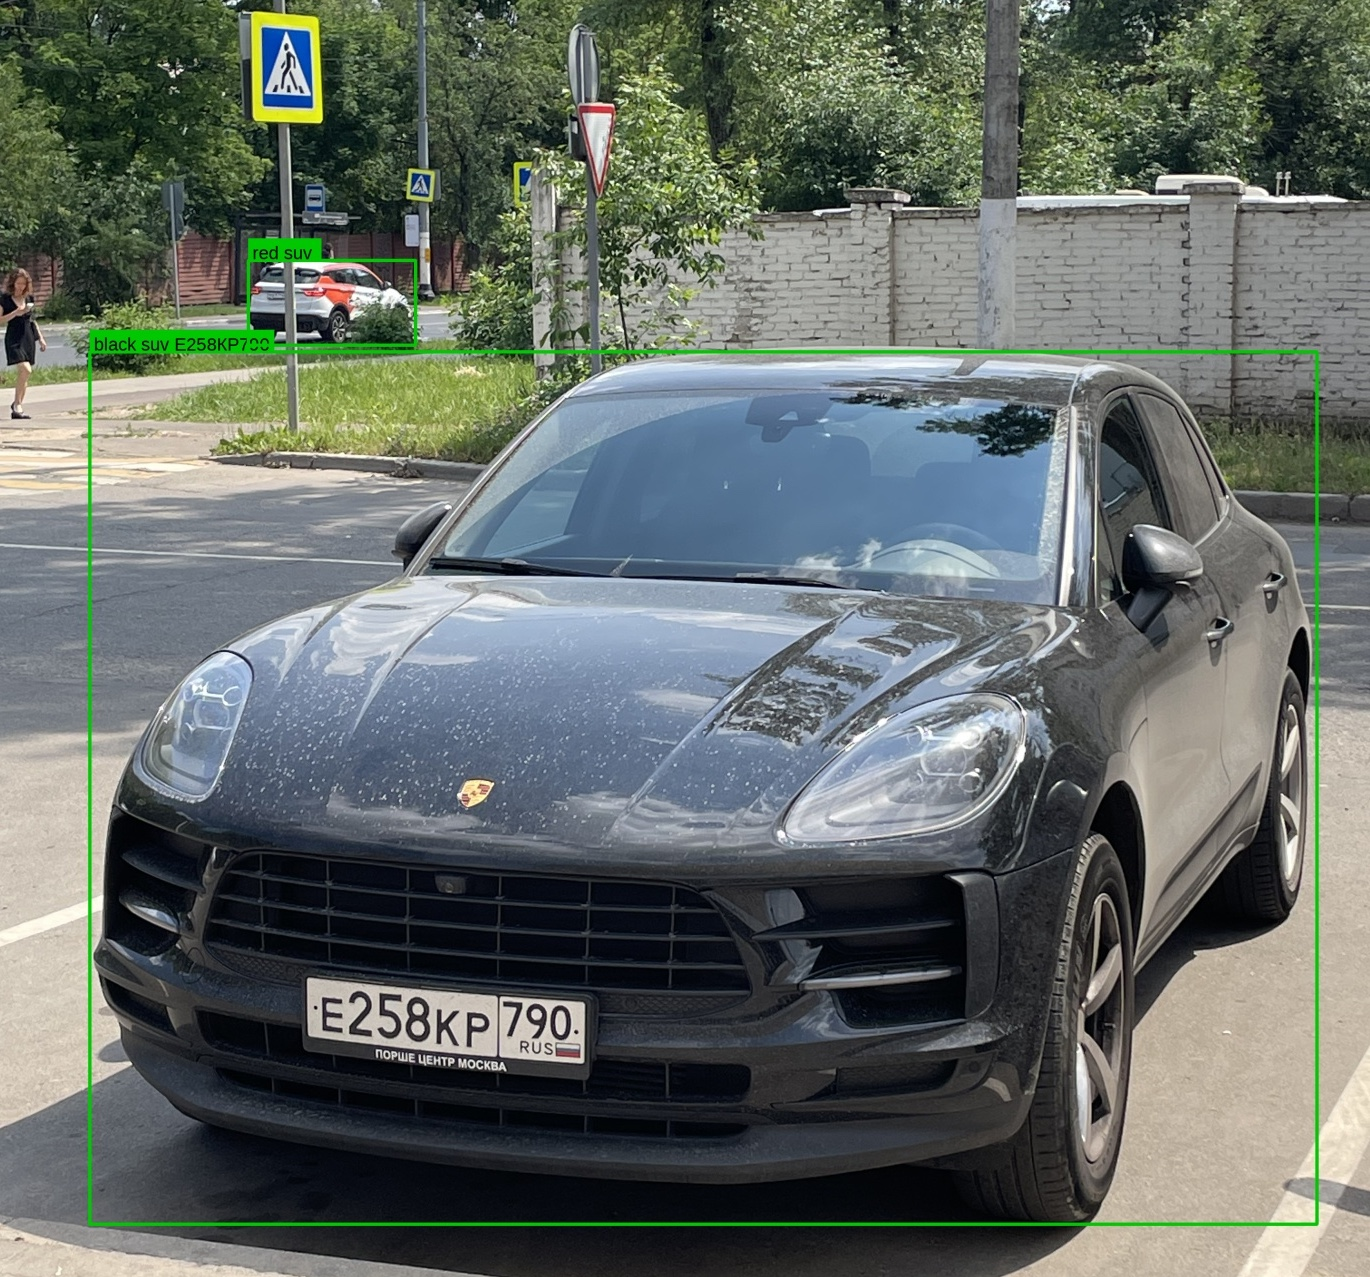
\includegraphics[height=5.8cm]{inf1.jpg}\caption{Porsche Macan}
\end{subfigure}\hfill
\begin{subfigure}{0.49\textwidth}\centering
  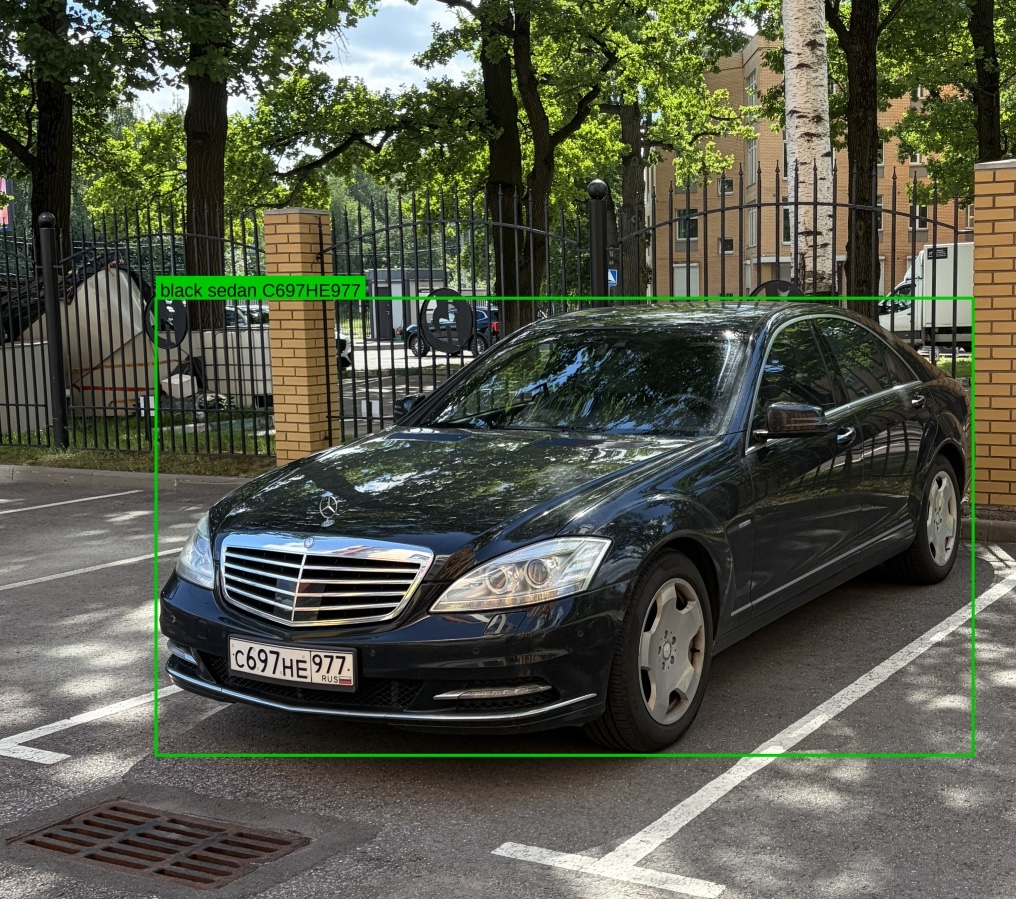
\includegraphics[height=5.8cm]{inf2.jpg}\caption{Mercedes-Benz S-класс}
\end{subfigure}

\medskip
\begin{subfigure}{0.7\textwidth}\centering
  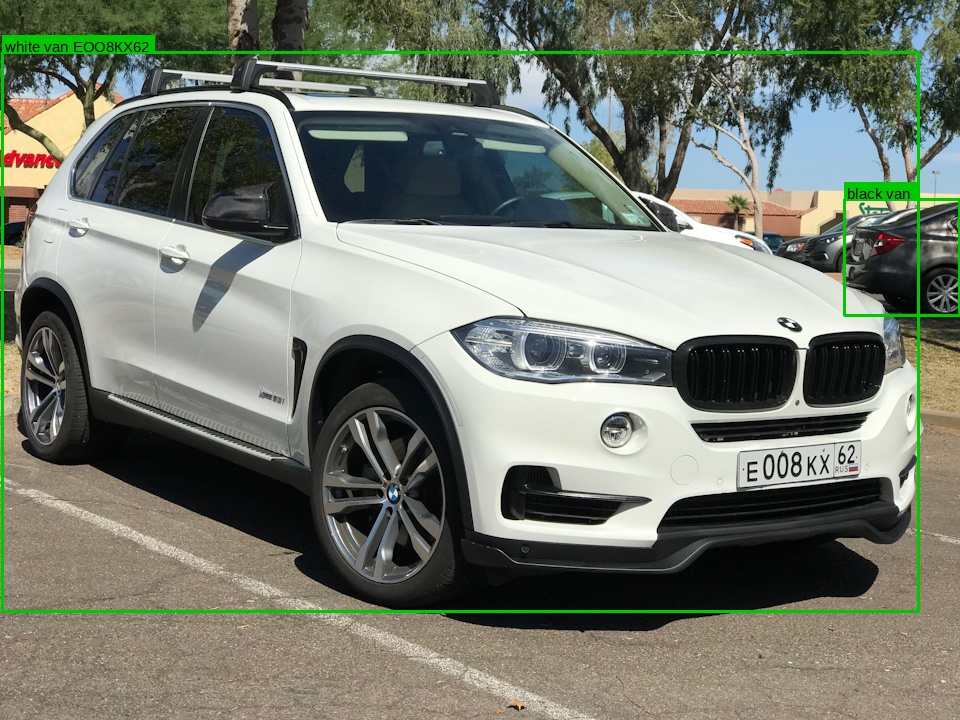
\includegraphics[height=4.8cm]{inf3.jpg}\caption{BMW X5}
\end{subfigure}
\caption{Результаты конвейера на одиночных изображениях: рамка ТС
с подписью «цвет~+ тип кузова~+ номер»}
\label{fig:single_infer}
\end{figure}

\begin{table}[H]
\centering
\caption{Предсказания конвейера на тестовых изображениях}
\label{tab:single_infer}
\rowcolors{2}{rowgray}{white}
\begin{tabular}{lccc}
\toprule
\textbf{ТС} & \textbf{Цвет} & \textbf{Тип кузова} & \textbf{Номер РФ} \\
\midrule
BMW X5          & white~(верно)  & suv~(верно)       & ЕОО8КХ62~(неверно)\textsuperscript{$\dagger$} \\
Porsche Macan   & black~(верно)  & suv~(верно)       & Е258КР790~(верно) \\
Mercedes-Benz S & black~(верно)  & sedan~(верно)     & С697НЕ977~(верно) \\
\midrule
\textbf{Итого}  & \textbf{3/3} & \textbf{3/3} & \textbf{2/3} \\
\bottomrule
\end{tabular}
\end{table}

\noindent\textsuperscript{$\dagger$}\,На BMW~X5 распознано «ЕОО8КХ62»:
две цифры «0» прочитаны как буква «О» (самая частая ошибка OCR,
O\,↔\,0, таблица~\ref{tab:ocr_confusions}). Визуально строка читается
корректно, но точного совпадения нет.

\textbf{Цвет (3/3).} Классификатор не ошибся ни на одном снимке~---
включая два тёмных бликующих кузова (Mercedes, Macan) и белый
BMW~X5. Это хорошо согласуется с заявленной
устойчивостью модели цвета (top-1\,=\,0.936,
таблица~\ref{tab:final_summary}) к реальному освещению и засветкам.

\textbf{Номер (2/3).} Точно прочитаны два номера:
Е258КР790 (Macan) и С697НЕ977 (Mercedes). Везде это
крупные фронтальные пластины ($\approx$200--300~px по ширине), то есть
для OCR условия близки к идеальным
(подраздел~\ref{subsec:ocr_errors}). Сбой произошёл лишь на BMW~X5: два
нуля распознаны как буква «О» (O\,↔\,0). Латинские гомоглифы в подписях
(Е/К/Х/С/Н/О/Р выводятся как E/K/X/C/H/O/P) носят чисто косметический
характер и смысл номера не меняют.

\textbf{Тип кузова (3/3).} Все три кузова определены верно: седан
(Mercedes~S) и внедорожники (BMW~X5, Porsche~Macan). Результат
укладывается в задокументированную
точность top-1\,=\,0.830 (таблица~\ref{tab:final_summary}): на крупных,
хорошо освещённых фронтальных кадрах, близких по ракурсу к обучающим,
модель уверенно разводит даже соседние формы. Стоит отметить, что
неудобная пара \emph{sedan\,↔\,hatchback} на валидации
(таблица~\ref{tab:body_per_class}) остаётся главным источником
путаниц, однако на крупных фронтальных кадрах данного теста седан
Mercedes~S разведён уверенно.

В итоге тест на одиночных кадрах демонстрирует, что на реальных данных
все три модуля работают согласованно: цвет и тип кузова угаданы на всех
трёх снимках, номер~--- на двух из трёх (единственный промах~--- O\,↔\,0). Оговоримся, что
кадры сняты в удобных условиях~--- крупный фронтальный ракурс, хорошее
освещение; доводка классификатора кузова под произвольные уличные
ракурсы и трудную пару sedan\,↔\,hatchback вынесена в задачи дальнейшей
адаптации к новым условиям.

\subsection{Видеоинференс с трекингом и покадровой агрегацией характеристик}
\label{subsec:video_tracking}

Базовый конвейер обрабатывает каждый кадр независимо. На видео это
порождает две проблемы: одна машина попадает в сотни кадров и даёт
столько же независимых детекций, а предсказания цвета, кузова и номера
«дрожат» от кадра к кадру. На тестовом ролике ($1280\times720$,
359~кадров) счётчик «распознанных» номеров вдобавок завышается
строками-обрезками неудачного OCR, не валидными по формату~РФ.

Для устранения этого реализован видеоинференс с межкадровым
сопровождением объектов алгоритмом ByteTrack (метод \texttt{track}
библиотеки Ultralytics): каждому ТС присваивается устойчивый
идентификатор, а характеристики накапливаются по треку, а не по кадрам:
\begin{itemize}[nosep]
  \item \textbf{цвет}~--- взвешенное по уверенности голосование softmax
    по крупным кадрам (сторона бокса $\geq$\,80~px);
  \item \textbf{тип кузова}~--- усреднение softmax по кадрам со стороной
    $\geq$\,128~px, с пометкой неуверенных предсказаний (порог 0.45);
  \item \textbf{номер}~--- наиболее частый среди \emph{формат-валидных}
    результатов OCR с кропов шириной $\geq$\,60~px (фолбэк на первые
    символы неудачной строки удалён).
\end{itemize}

Для цвета и чтения номера выбирается «лучший» кадр трека по резкости
(дисперсия лапласиана), а гейтинг по размеру отсекает мелкие и тёмные
кадры. Это снимает систематическую ошибку, когда усреднение по всем
кадрам «топило» немногочисленные чёткие кадры в массе тёмных и смазанных;
после агрегации цвет обоих подъехавших вблизи автомобилей (чёрного BMW и
белого седана) определён устойчиво (таблица~\ref{tab:video_tracks}).

Проявляется и порог читаемости номера по разрешению кропа: два
подъехавших близко автомобиля распознаны верно (BMW~--- А356КН550,
такси~--- В431УЕ169, обе строки прошли формат-валидацию), а у более
удалённых ТС ширина кропа осталась ниже порога $\gtrsim$\,80~px
(подраздел~\ref{subsec:ocr_errors}). Ограничение для дальних номеров
носит физический характер (разрешение), а не алгоритмический.

\begin{table}[H]
\centering
\caption{Результаты видеоинференса для двух подъехавших вплотную ТС
на тестовом ролике ($1280\times720$, 359~кадров)}
\label{tab:video_tracks}
\rowcolors{2}{rowgray}{white}
\begin{tabular}{lccc}
\toprule
\textbf{ТС} & \textbf{Цвет} & \textbf{Тип кузова} & \textbf{Номер РФ} \\
\midrule
BMW X1    & black~(верно) & suv~(верно) & А356КН550~(верно) \\
Kia Rio         & white~(верно) & suv~(неверно)\textsuperscript{$\dagger$} & В431УЕ169~(верно) \\
\bottomrule
\end{tabular}
\end{table}

\noindent\textsuperscript{$\dagger$}\,Седан-такси принят за \textit{suv}~---
классификатор кузова путает близкие формы (пара
\textit{sedan}\,↔\,\textit{suv}\,↔\,\textit{hatchback} остаётся основным
источником ошибок, таблица~\ref{tab:body_per_class}). Цвет и
номер у обоих ТС определены верно. Помимо этих двух машин конвейер
сопровождал и другие проезжавшие ТС (белый седан, серебристый кроссовер,
удалённый поток), но их номерные пластины остались ниже порога читаемости.

\begin{figure}[H]
\centering
\begin{subfigure}{0.49\textwidth}\centering
  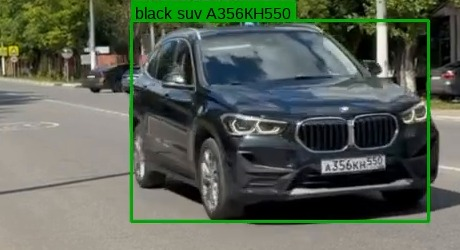
\includegraphics[width=\textwidth]{vid_bmw.jpg}
  \caption{BMW X1: black\,/\,suv\,/\,А356КН550}
\end{subfigure}\hfill
\begin{subfigure}{0.49\textwidth}\centering
  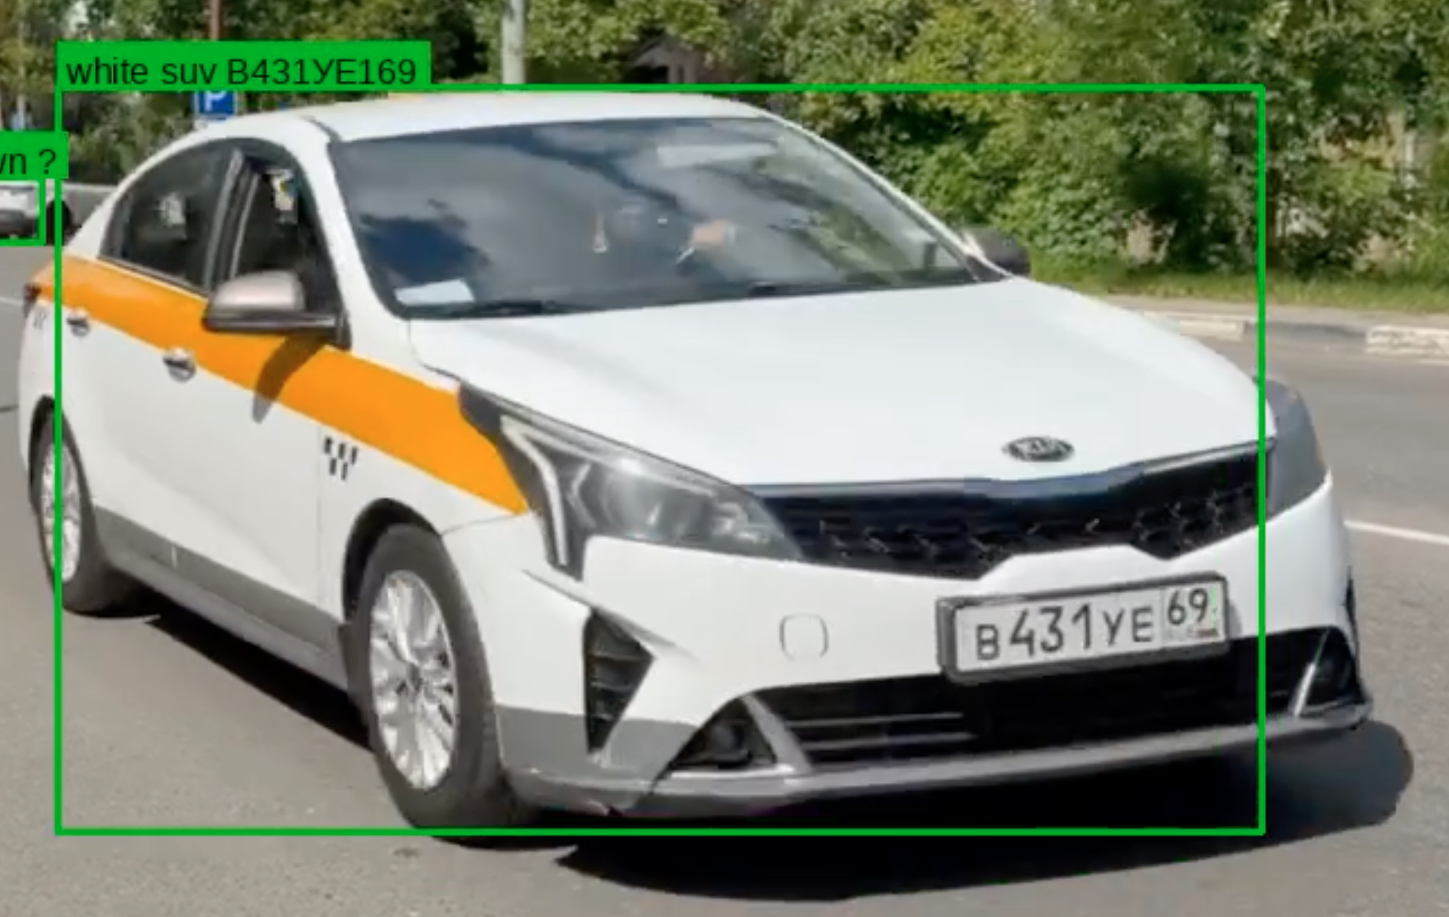
\includegraphics[width=\textwidth]{vid_taxi.jpg}
  \caption{Kia Rio: white\,/\,В431УЕ169}
\end{subfigure}
\caption{Кадры размеченного видео с устойчивой по треку подписью
«цвет\,+\,тип кузова\,+\,номер». У обоих подъехавших вплотную ТС цвет и
номер РФ распознаны верно}
\label{fig:video_annotated}
\end{figure}

Результат сохраняется как размеченное видео с устойчивой по объекту
подписью «цвет~+ тип кузова~+ номер» (вместо мерцающих покадровых меток)
и галерея по одной карточке на каждое ТС. Агрегация сворачивает сотни
покадровых детекций к числу реальных объектов: у двух подъехавших на
читаемую дистанцию ТС цвет и номер РФ определены верно, тогда как тип
кузова у такси ошибочен (седан принят за \textit{suv}). Оставшиеся
ограничения носят модельный характер: слабость классификатора кузова на
нефронтальных ракурсах, отсутствие класса \textit{gray} и физический
предел разрешения для удалённых номеров.

\subsection{Метрики производительности}

\begin{table}[H]
\centering
\caption{Задержка и производительность модулей конвейера (GPU~T4)}
\label{tab:pipeline_fps}
\rowcolors{2}{rowgray}{white}
\begin{tabular}{lcc}
\toprule
\textbf{Модуль} & \textbf{Задержка, мс} & \textbf{Доля, \%} \\
\midrule
YOLO26n детекция ТС       & 13 & 3 \\
YOLO26n детекция номера   & 13 & 3 \\
ResNet18 цвет             & 3  & 1 \\
ResNet18 кузов            & 3  & 1 \\
EasyOCR (кроп номера)     & $\approx$350--500 & 92 \\
\midrule
\textbf{Итого (pipeline)} & $\approx$400 & 100\% \\
\textbf{FPS (без OCR)}    & \multicolumn{2}{c}{$\approx$30} \\
\bottomrule
\end{tabular}
\end{table}

\subsection{Итоговая таблица результатов}

\begin{table}[H]
\centering
\caption{Сводная таблица метрик по всем модулям}
\label{tab:final_summary}
\rowcolors{2}{rowgray}{white}
\begin{tabularx}{\textwidth}{lXcX}
\toprule
\textbf{Модуль} & \textbf{Компонент} & \textbf{Метрика} & \textbf{Результат} \\
\midrule
Детекция ТС         & YOLO26n (COCO pretrained)  & mAP@0.5:0.95   & 0.409 (COCO val) \\
Детекция номеров    & \textbf{YOLO26n (fine-tuned)} & \textbf{mAP@0.50} & \textbf{0.9669} \\
Классификация цвета & ResNet18 (VCoR)            & Accuracy top-1 & \textbf{0.936} \\
Классификация цвета & ResNet18 (VCoR)            & Accuracy top-3 & 0.993 \\
Классификация кузова& ResNet18 (CompCars)        & Accuracy top-1 & \textbf{0.830} \\
OCR (NOMEROFF-NET RU) & EasyOCR ru+en           & CRR / Plate Acc & 0.750 / 0.225 \\
\textbf{Pipeline}   & \textbf{Конвейер (без OCR)} & \textbf{FPS}  & $\approx$\textbf{30} \\
\bottomrule
\end{tabularx}
\end{table}

\subsection{Детальный анализ ошибок OCR}
\label{subsec:ocr_errors}

\textbf{Протокол оценки.}
EasyOCR (модель \texttt{ru+en}) оценивался на 200 случайно выбранных
кропах из NOMEROFF-NET~RU~--- реальные фотографии с улицы
(2845~пар image/GT в датасете).
Метрики: Plate\,Accuracy (совпадение всей строки целиком) и
CRR~$=1-\mathrm{CER}$, где $\mathrm{CER}$~--- Character Error Rate
по алгоритму Левенштейна.

\textbf{Результаты.}
На реальных кропах: Plate\,Acc~$=0.225$, CRR~$=0.750$.
Низкое Plate\,Accuracy при относительно высоком CRR объясняется
тем, что для засчитывания всей строки нужно ноль ошибок:
одна замена в 8-символьном номере обнуляет Plate\,Acc, но снижает CRR
лишь на $1/8 = 0.125$.

\textbf{Топ замен символов (NOMEROFF-NET RU, 200 кропов).}

\begin{table}[H]
\centering
\caption{Наиболее частые пары замен символов в OCR (кириллица/цифра)}
\label{tab:ocr_confusions}
\rowcolors{2}{rowgray}{white}
\begin{tabular}{ccc p{7cm}}
\toprule
\textbf{GT} & \textbf{Pred} & \textbf{Кол-во} & \textbf{Причина} \\
\midrule
О & 0 & 26 & Круглая форма; кириллическая «О» против арабского нуля \\
В & 8 & 17 & Схожие замкнутые контуры \\
А & 4 & 12 & Угловая форма; верхняя перекладина «А» схожа с «4» \\
Т & 7 & 8  & Горизонтальная черта «Т» при малом разрешении \\
У & 7 & 8  & Угловой нижний штрих «У» схож с «7» \\
О & 9 & 8  & Неполное замыкание контура из-за шума \\
3 & 5 & 6  & Схожие изогнутые сегменты \\
7 & 8 & 6  & Горизонтальная перекладина «8» против штриха «7» \\
\bottomrule
\end{tabular}
\end{table}

Все 8 наиболее частых ошибок относятся к парам \emph{кириллица~↔~цифра}
или \emph{визуально похожие глифы}.
Это объясняется тем, что EasyOCR обучался на общем корпусе текстов,
где кириллические и латинские буквы встречаются гораздо реже
в соседстве с цифрами. Специализированные CRNN-модели для номеров
(например, LPRNet) дообучаются именно на таких парах и показывают
CRR~$>0.97$ на аналогичных реальных данных.

\textbf{Факторы, ограничивающие точность OCR.}
Основные причины ошибок на реальных уличных кропах:
\begin{itemize}[nosep]
  \item \textbf{Угол съёмки:} перспективное искажение сжимает символы,
    особенно боковые; детектор CRAFT хуже локализует границы символов;
  \item \textbf{Разрешение:} при расстоянии $>15$~м кроп номера
    содержит менее 80 пикселей в ширину против 200--300 пикселей
    при съёмке вблизи;
  \item \textbf{Освещение и блики:} засветка рефлектирующих пластин
    в ярком солнечном свете или ночью при фарах встречного транспорта
    частично скрывает контуры символов.
\end{itemize}

\subsection{Анализ узких мест и практические рекомендации}

\textbf{Узкое место~--- EasyOCR.}
EasyOCR выполняет два прохода по изображению (CRAFT для
детекции символьных регионов + CRNN+CTC для декодирования строки)
на CPU, что и объясняет задержку 350--500 мс. Без OCR конвейер
работает в реальном времени ($\approx$30 FPS), что достаточно
для обработки стандартных 25-FPS видеопотоков.

\textbf{Влияние резолюции номерного знака.}
EasyOCR наиболее чувствителен к разрешению кропа номерного знака.
При разрешении входного кадра 1080p кроп номера содержит $\approx$200--300
пикселей в ширину~--- достаточное разрешение для устойчивого OCR. При разрешении
ниже 720p качество OCR существенно снижается~--- это типичная проблема
для камер с низким разрешением.

\textbf{Стратегии ускорения OCR:}
\begin{enumerate}[nosep]
  \item Замена EasyOCR на CRNN, оптимизированный для российских
    номеров~--- даст $\approx$5--10$\times$ ускорение;
  \item Запуск EasyOCR на GPU: при наличии достаточной памяти
    задержка снижается до 50--80 мс;
  \item покадровая агрегация по сопровождаемым объектам с чтением номера
    только по «лучшим» кадрам трека~--- реализована в данной работе
    (подраздел~\ref{subsec:video_tracking}): снижает число вызовов OCR и
    устраняет мерцание предсказаний.
\end{enumerate}

\textbf{Качественный результат на одиночных изображениях.}
На трёх тестовых фотографиях (подраздел~\ref{subsec:single_image})
конвейер верно определил цвет и тип кузова у всех трёх ТС (3/3 и 3/3)
и точно распознал номер у двух из трёх (2/3; единственная ошибка~---
путаница O\,↔\,0). Снимки сделаны в благоприятных условиях (крупный
фронтальный ракурс, хорошее освещение); это подтверждает согласованную
работу всех трёх модулей в режиме end-to-end, а повышение устойчивости
классификатора кузова к произвольным уличным ракурсам отнесено к
направлениям дальнейшей адаптации к новым условиям.

%% =============================================================
%%  ГЛАВА 4 --- ЗАКЛЮЧЕНИЕ
%% =============================================================
\chapter*{Заключение}
\addcontentsline{toc}{chapter}{Заключение}

В ходе выпускной квалификационной работы достигнута поставленная цель~---
разработана система автоматического определения характеристик транспортных
средств (номерной знак, цвет кузова, тип кузова) по видеопотоку. Все шесть
задач, сформулированных во введении, выполнены:
проведён анализ существующих методов детекции и классификации, обоснован
выбор архитектур, подготовлены датасеты, обучены и оценены модели,
реализован единый конвейер обработки видео, проведён сравнительный
эксперимент ResNet18, ResNet50 и EfficientNet-B0. Основные результаты приведены ниже.

\begin{enumerate}
  \item \textbf{Архитектурный выбор.}
        Комбинация YOLO26n~+ ResNet18~+ EasyOCR обеспечивает приемлемый баланс
        точности и скорости (см. таблицу~\ref{tab:final_summary}).

  \item \textbf{Детектор номерных знаков.}
        Дообучение YOLO26n на датасете Russian license plates (Kaggle,
        668 изображений, 50 эпох, batch=16, \texttt{optimizer=auto})
        подняло mAP@0.50 до \textbf{0.9669} против $\approx$0.503 у
        исходной COCO-модели. В роли финального детектора (и ТС, и
        номеров) оставлен YOLO26n как более выгодная архитектура: имея
        меньше параметров (2.4M против 3.2M у YOLOv8n), меньшую
        вычислительную сложность и сквозной инференс без NMS, он
        одновременно точнее как на эталонном COCO, так и на целевых
        данных (mAP@0.50\,=\,0.9669 против 0.9554 у дообученного в тех же
        условиях YOLOv8n). Этот результат лишний раз показывает, насколько
        эффективен transfer learning при скромном объёме целевых данных.

  \item \textbf{Классификация цвета.}
        ResNet18 после 20 эпох двухфазного дообучения на VCoR выходит на
        Accuracy top-1\,=\,\textbf{0.936} и top-3\,=\,0.993. Тяжелее всего
        дались \textit{silver} (F1\,=\,0.867) и \textit{orange}
        (F1\,=\,0.896)~--- оба путаются с соседними цветами при разном
        освещении. По сравнению с кластеризационными методами выигрыш
        составляет 7--12\,\% (таблица~\ref{tab:color_methods}).

  \item \textbf{Классификация типа кузова.}
        ResNet18 (полное двухфазное дообучение, очищенная разметка
        sedan, аугментации под уличные сцены и TTA) достигает
        Accuracy top-1\,=\,\textbf{0.830} и top-3\,=\,0.969.
        Сравнение архитектур в едином режиме feature extraction
        (таблица~\ref{tab:arch_comparison}) показало, что наибольшую
        точность даёт ResNet50 (0.652), однако ResNet18 опережает
        её по скорости более чем вдвое (340.6 против 165.3~FPS на GPU~T4)
        при отставании в точности всего на 7~п.п.; поэтому для
        реального видеоконвейера выбрана ResNet18. Характерно, что
        EfficientNet-B0 при наименьших FLOPS (0.39G) оказалась самой
        медленной (84.4~FPS): depthwise-свёртки слабо утилизируют GPU.
        Наиболее сложный класс~--- \textit{hatchback} (F1\,=\,0.694)
        из-за визуального сходства с седаном.

  \item \textbf{OCR номерных знаков.}
        На реальных кропах NOMEROFF-NET~RU (200 изображений из 2845)
        EasyOCR обеспечивает Plate\,Acc\,=\,0.225 и CRR\,=\,0.750.
        Анализ ошибок выявил
        основные пары путаниц: О↔0 (26 случаев), В↔8 (17), А↔4 (12),
        Т↔7 (8), У↔7 (8)~--- все являются визуально схожими символами.
        Основные ошибки обусловлены
        неидеальным освещением, ракурсом и разрешением номеров на улице.

  \item \textbf{Производительность конвейера.}
        Блоки детекции и классификации на GPU~T4 суммарно дают
        $\approx$\,30~FPS. Узкое место~--- EasyOCR ($>$\,90\,\%
        от общего времени). Без OCR конвейер работает в реальном
        времени (таблица~\ref{tab:pipeline_fps}).

  \item \textbf{Видеоинференс с агрегацией по объектам.}
        Над покадровым конвейером надстроено сопровождение машин
        (ByteTrack): характеристики копятся по каждому треку~---
        голосованием для цвета и типа кузова и выбором самого частого
        формат-валидного номера. Так уходит мерцание предсказаний, сотни
        покадровых детекций сворачиваются к числу реальных объектов, а у
        подъехавших вплотную ТС на тестовом ролике (359~кадров) верно
        прочитаны два номера РФ; метрика распознанных
        номеров становится честной. Опытным путём найден порог
        читаемости~--- кроп номера шириной $\gtrsim$\,80~px
        (подраздел~\ref{subsec:video_tracking}).

  \item \textbf{Ограничения системы.}
        Главным узким местом конвейера остаётся EasyOCR; разумно
        перейти на отдельный облегчённый OCR-модуль.
\end{enumerate}

\textbf{Направления дальнейшего развития:}
\begin{itemize}[nosep]
  \item замена EasyOCR на CRNN-детектор, оптимизированный для российских номеров;
  \item расширение классов цвета и типа кузова;
  \item адаптация к ночным условиям съёмки (low-light enhancement).
\end{itemize}

%% =====================  ЛИТЕРАТУРА  =========================
\addcontentsline{toc}{chapter}{Список использованных источников}
\begin{thebibliography}{99}

\bibitem{survey2021}
Lubna, Mufti N., Shah S.\,A.\,A.
\textit{Automatic Number Plate Recognition: A Detailed Survey of Relevant Algorithms}~//
Sensors, 21(9):3028, 2021.

\bibitem{yolo26}
Ultralytics.
\textit{YOLO26: Key Architectural Enhancements and Performance Benchmarking
for Real-Time Object Detection}~// arXiv:2509.25164, 2025.
URL: \url{https://docs.ultralytics.com/models/yolo26}.

\bibitem{laroca2018}
Laroca R., Severo E., Zanlorensi L.\,A. и др.
\textit{A Robust Real-Time Automatic License Plate Recognition Based on the YOLO Detector}~//
arXiv:1802.09567, 2018.

\bibitem{laroca2021}
Laroca R., Zanlorensi L.\,A., Gonçalves G.\,R. и др.
\textit{An Efficient and Layout-Independent Automatic License Plate Recognition System Based on the YOLO Detector}~//
IET Intelligent Transport Systems, 15(4):483--503, 2021.

\bibitem{vmmr2024}
\textit{Two decades of vehicle make and model recognition}~//
Journal of King Saud University~--- CIS, 2024.

\bibitem{siddiqui2016}
Siddiqui A., Mammeri A., Boukerche A.
\textit{Real-Time Vehicle Make and Model Recognition Based on SURF Features}~//
IEEE ITS, 2016.

\bibitem{manzoor2022}
Manzoor M.\,A., Morgan Y., Bais A.
\textit{Real-Time Vehicle Make and Model Recognition System}~//
Machine Learning and Knowledge Extraction, 1(2):611--629, 2019.

\bibitem{su2015}
Rachmadi R.\,F., Purnama I.\,K.\,E.
\textit{Vehicle Color Recognition using Convolutional Neural Network}~//
arXiv:1510.07391, 2015.

\bibitem{kubatin2019}
Кубатин И.\,А.
\textit{Алгоритм определения цвета автомобиля с использованием метода k-средних}~//
КиберЛенинка, 2019.

\bibitem{zhang2018mixup}
Zhang H., Cisse M., Dauphin Y.~N., Lopez-Paz D.
\textit{mixup: Beyond Empirical Risk Minimization}~//
ICLR, 2018.

\bibitem{he2016resnet}
He K., Zhang X., Ren S., Sun J.
\textit{Deep Residual Learning for Image Recognition}~//
IEEE CVPR, 2016.~--- P.~770--778.

\bibitem{tan2019efficientnet}
Tan M., Le Q.\,V.
\textit{EfficientNet: Rethinking Model Scaling for Convolutional Neural Networks}~//
ICML, 2019.~--- P.~6105--6114.

\bibitem{hu2018senet}
Hu J., Shen L., Sun G.
\textit{Squeeze-and-Excitation Networks}~//
IEEE CVPR, 2018.~--- P.~7132--7141.

\end{thebibliography}

\end{document}